% ************************* Preámbulo ********************************

% *************** Document Class ***************
% Para más información sobre las clases:
% https://en.wikibooks.org/wiki/LaTeX/Document_Structure#Document_classes
% En la tabla "Document classes"
% https://ctan.org/topic/class
% \documentclass[10pt, a4paper]{book}
\documentclass[12pt, twoside, a4paper, openright]{book} % \documentclass[options]{class}
% Si usas twoside en vez de oneside, LaTeX te pondrá hojas blancas adicionales

% Para más información sobre las opciones:
% https://en.wikibooks.org/wiki/LaTeX/Document_Structure#Document_classes
% En la tabla "Document Class Options"

% Posibles opciones:
% 10pt, 11pt, 12pt : El tamaño de la fuente por defecto
% a4paper, letterpaper,... : El tamaño del papel del documento
% twocolumn
% landscape
% titlepage, notitlepage
% openright, openany
% draft
% fleqn
% leqno

%------------ Paquetes, macros y metadata ------------%
% ************************ Thesis Information & Meta-data **********************

%------------Información básica------------%
\newcommand{\egilea}{Baldwin David Rodr\'{i}guez Ponce} % The full name of the author
\newcommand{\zuzendariak}{Mar\'{i}a Begoña Losada Pereda}

\newcommand{\upvehu}{Universidad del País Vasco UPV/EHU} % University
\newcommand{\informatikafakultatea}{Facultad de Informática}
\newcommand{\gradua}{Grado en Ingeniería Informática}  % Full title of the Degree
\newcommand{\espezialitatea}{Computación}

\newcommand{\izenburua}{Transpilador de un lenguaje de modelado personalizado de sistemas de simulación dinámicos discretos a
Python} % The title of the thesis
% \newcommand{\izenburua}{Simpy: Un lenguaje de modelado de sistemas de simulación dinámicos discretos} % The title of the thesis
\newcommand{\gapizenburua}{Trabajo de Fin de Grado} % Subtitle
% \newcommand{\gapizenburua}{Proyecto de Fin de Grado}

\newcommand{\crest}{\includegraphics[width=0.6\textwidth]{1-Portada/FacultadInformatica.jpg}} % University Crest (logo)
\newcommand{\data}{\today} % Submission date
\newcommand{\urtea}{2022}

\newcommand{\egileatestua}{Autor}
\newcommand{\zuzendariaktestua}{Directora}

\newcommand{\abstract}{Resumen}

\message{LaTeX Warning: \noexpand Aviso! Mejor si cambias los textos `Autor/a' y `Directore/a (s)' en funcion del numero y el genero!}

 % Metadata
% ################################################################
% #######     CODIFICACIÓN DEL ARCHIVO              ##############
% ################################################################

% ************************* Input encoding ********************************
% \usepackage{ucs}
\usepackage[utf8]{inputenc} % Permite usar carácteres UTF8
% https://www.overleaf.com/learn/latex/Spanish

% ************************* Output encoding ********************************
\usepackage[T1]{fontenc} % Use 8-bit encoding that has 256 glyphs
% https://www.overleaf.com/learn/latex/Spanish
% \usepackage{courier}

% ************************* Font types ********************************
% times erabili beharrean
\usepackage{mathptmx}
\usepackage[scaled=.90]{helvet}

% ************************* Lenguaje a utilizar ********************************

\usepackage[spanish, es-tabla]{babel} %To extend the default capabilities of LaTeX, providing proper hyphenation and translation of the names of document elements.
% https://www.overleaf.com/learn/latex/Spanish
% \usepackage{hyphenat} % Paquete para controlar la separación de palabras
% \hyphenation{mate-máti-cas recu-perar}



% ################################################################
% #######              GEOMETRY                     ##############
% ################################################################

% ************************* Geometría ********************************
% \usepackage[a4paper, inner=1.5cm, outer=3cm, top=4cm, bottom=3cm, bindingoffset=1cm]{geometry}
% \usepackage[a4paper, left=37mm,right=30mm,top=35mm,bottom=30mm]{geometry}
% \usepackage[left=2.5cm, right=3.5cm, top=4.0cm, bottom=3.0cm]{geometry}
\usepackage[a4paper, inner=2.0cm, outer=3.5cm, top=4.0cm, bottom=3.0cm, marginpar=2.0cm, headheight=14.5pt, showframe]{geometry}

% use option "showframe" in geometry to see frames
% \usepackage[showframe]{geometry}

% ************************* Layout visualization ********************************

\usepackage{layout} % To see the layout of the page
% \usepackage{showframe}


% ################################################################
% #######     ESTILOS EN GENERAL                    ##############
% ################################################################

% *********************** Cabeceras ******************************
\usepackage{fancyhdr} % Permite cambiar el estilo de las cabeceras y pies de página de las páginas del documento
% https://ctan.javinator9889.com/macros/latex/contrib/fancyhdr/fancyhdr.pdf

% \usepackage{fncychap} % Este paquete permite cambiar el estilo de la cabecera de los capítulos
\usepackage[sf,outermarks]{titlesec} % Este paquete permite cambiar el estilo de las cabeceras, pies de página y la forma de las secciones y divisores de sección.
% \usepackage[compact]{titlesec}
% \usepackage{sectsty}


% ************************* ToC and Index ********************************
\usepackage[nottoc]{tocbibind} % Para añadir las listas de figuras y cuadros a la TOC
% \usepackage[acronym,footnote,nonumberlist,toc]{glossaries}
% Erabilera
% http://en.wikibooks.org/wiki/LaTeX/Glossary
% latexmk erabiliz gero, ikusi http://tex.stackexchange.com/questions/1226/how-to-make-latexmk-use-makeglossaries

% Glosario-en eskuliburu zabaldua
% http://osl.ugr.es/CTAN/macros/latex/contrib/glossaries/glossaries-user.html#x1-140002.2
\usepackage[page]{appendix} % Añade el enviroment appendices
% \usepackage[toc,page]{appendix} % Añade una tabla de apéndices a la ToC
% https://osl.ugr.es/CTAN/macros/latex/contrib/appendix/appendix.pdf
% \addto{\captionsspanish}{
%     \renewcommand*{\appendixpagename}{Ap\'{e}ndices}
%     \renewcommand*{\appendixtocname}{Ap\'{e}ndices}
% }
\usepackage{makeidx} % Para crear el index si existe

% *********************** Global paragraph indentation ******************************
\usepackage{parskip} % El único propósito es quitar el indent de todos los párrafos
\usepackage{setspace} % spacing environment
%\usepackage[protrusion=true,expansion=true]{microtype}



% ################################################################
% #######     COLOURS                               ##############
% ################################################################

% *************************** Colours *****************************

\usepackage{color}
\usepackage[table, svgnames, pdftex,dvipsnames]{xcolor} %  Coloured text etc.
% https://ctan.javinator9889.com/macros/latex/contrib/xcolor/xcolor.pdf
\usepackage{colortbl}



% ################################################################
% #######     GRAPHICS                              ##############
% ################################################################

% *************************** Graphics and figures *****************************
\usepackage{epsf, graphics, graphicx}

\usepackage[figuresright]{rotating}
%\usepackage{wrapfig}

\usepackage{float} % Fuerza las figuras a una posición exacta

\usepackage[font=small,labelfont=bf]{caption}
\usepackage{subcaption} % Permite poner subsubtítulos dentro de figuras compuestas
% http://mirrors.ibiblio.org/CTAN/macros/latex/contrib/caption/subcaption.pdf

% \usepackage{tikz} % Advanced inline graphics.
% % https://www.bu.edu/math/files/2013/08/tikzpgfmanual.pdf
% % https://ctan.javinator9889.com/graphics/pgf/base/doc/pgfmanual.pdf
% \usepackage{pgfplots}
% \usetikzlibrary{shapes, decorations, calc, arrows}
% \usetikzlibrary{3d,fit,backgrounds, decorations.text}
% \usetikzlibrary{positioning, shapes.symbols}
% \usetikzlibrary{decorations.pathreplacing, calligraphy}
% \tikzset{>=latex}



% ################################################################
% #######     MATHEMATICS                           ##############
% ################################################################

% ************************* Mathematics ********************************
\usepackage{amsmath}
\usepackage{amssymb}
% \usepackage{amsthm} % Use ntheorem better
\usepackage{ntheorem} % Customizing and writing theorems
\usepackage{bm} % Bold math symbols
\usepackage{amscd}
\usepackage{latexsym} % Even more operators. http://mirrors.ibiblio.org/CTAN/macros/latex/base/latexsym.pdf
\usepackage{calc} % Para hacer cálculos de longitudes en los comandos

% *********************************** SI Units *********************************
\usepackage{siunitx} % use this package module for SI units


% ************************* Text typesetting extras ********************************
\usepackage{csquotes} % Para permitir citas en el texto (bonitas)
\usepackage{circledsteps} % Permite crear texto y números encerrados en círculos
% \usepackage[activate=true, final, tracking=true, kerning=true, spacing=true, factor=1100, stretch=10, shrink=10]{microtype}
% \usepackage{microtype}

\usepackage{lipsum}                     % Dummytext
\usepackage{xargs}                      % Use more than one optional parameter in a new commands

% ################################################################
% #######     INSERTABLES                           ##############
% ################################################################

% ************************* Beatiful colorboxes (breakable) ********************************
% \usepackage{mdframed}
\usepackage[most]{tcolorbox} % https://osl.ugr.es/CTAN/macros/latex/contrib/tcolorbox/tcolorbox.pdf

% ******************************* Itemize and enumerate *********************************

\usepackage{paralist} % compactenum...
\usepackage{enumitem} % Customizable enums
% https://ctan.javinator9889.com/macros/latex/contrib/enumitem/enumitem.pdf

% ******************************* Tables *********************************

% https://ctan.javinator9889.com/macros/latex/contrib/booktabs/booktabs.pdf
\usepackage{array} % For defining special column types
\usepackage{ragged2e} % For new types of columns
\usepackage{longtable} % For breakable tables
\usepackage{multirow} % Table cells that span multiple rows
\usepackage{multicol} % Table cells that span multiple columns
% https://osl.ugr.es/CTAN/macros/latex/required/tools/array.pdf
\usepackage{tabulary}
% https://osl.ugr.es/CTAN/macros/latex/contrib/tabulary/tabulary.pdf
% \usepackage{xltabular}
% https://www.ctan.org/pkg/xltabular
%\usepackage{tabularx}
% https://ctan.org/pkg/tabularx?lang=en
\usepackage{booktabs} % For professional looking tables

% *************************** Listings *****************************

% http://tug.ctan.org/tex-archive/macros/latex/contrib/caption/caption-eng.pdf
% \usepackage{listingsutf8} % - Para escribir código
\usepackage{listings}
% https://www.overleaf.com/learn/latex/Code_listing
% https://osl.ugr.es/CTAN/macros/latex/contrib/listings/listings.pdf

% \usepackage{minted} % Substitute for listings
% https://github.com/gpoore/minted/blob/master/source/minted.pdf
% \usepackage{textcomp} % XML kodea formateatzeko

% ************************* Margin Notes ********************************
\usepackage{marginnote}
\usepackage{marginfix}
% \usepackage{mparhack}

% *********************************** TODO Comments *********************************
% \setlength {\marginparwidth }{2cm}
\usepackage[colorinlistoftodos,prependcaption,textsize=scriptsize,textwidth=2cm]{todonotes}


% ################################################################
% #######     REFERENCES AND BIBLIOGRAPHY           ##############
% ################################################################

% ************************* Bibliography ********************************
\usepackage[backend=biber,style=apa,autocite=plain,sorting=ynt]{biblatex}

% ************************* Referencias y enlaces ********************************
\usepackage{url} % https://osl.ugr.es/CTAN/macros/latex/contrib/url/url.pdf

\usepackage[hyperindex,bookmarks,colorlinks=true,citecolor=blue,urlcolor=blue,linkcolor=blue,pdftex,unicode]{hyperref} % Se recomienda que sea el último paquete en ser importado

\usepackage{cleveref} % Clever references (éste debe ser en realidad el último paquete importado)

% line in order to check if utf-8 is properly configured: áéíóúñ
% ################################################################
% #######     CODIFICACIÓN DEL ARCHIVO              ##############
% ################################################################

% ************************* Input encoding ********************************

% ************************* Output encoding ********************************
\DeclareSymbolFont{usualmathcal}{OMS}{cmsy}{m}{n}
\DeclareSymbolFontAlphabet{\mathcal}{usualmathcal}

% ************************* Lenguaje a utilizar ********************************
\addto\captionsspanish{
	\renewcommand{\contentsname}{Tabla de contenidos}
	\renewcommand{\listtablename}{\'{I}ndice de tablas}
	\renewcommand{\listfigurename}{\'{I}ndice de figuras}
	\renewcommand{\lstlistlistingname}{\'{I}ndice de códigos}
	\renewcommand{\tablename}{Tabla}
	\renewcommand{\appendixname}{Anexo}
	\renewcommand{\appendixpagename}{Anexos}
	\renewcommand{\appendixtocname}{Anexos}
	\renewcommand{\lstlistingname}{Código} % Listing -> Listado
}
\input{0-Preambulo/macros/1-geometria}
% ################################################################
% #######     ESTILOS EN GENERAL                    ##############
% ################################################################

% *********************** Cabeceras ******************************

% ************ Headers, Footnotes and others ************
% % De las cabeceras y pies de página de cada página:
\fancypagestyle{empty}{ %
    \fancyhf{} % remove everything
    \renewcommand{\headrulewidth}{0pt} % remove lines as well
    \renewcommand{\footrulewidth}{0pt}
}

% Redefine plain page style
\fancypagestyle{plain}{
	\fancyhf{}
	\renewcommand{\headrulewidth}{0pt}
	\fancyfoot[LE,RO]{\thepage}
}

\fancypagestyle{fancy-intro}{%
    \fancyhf{}
    \fancyhead[RE]{\textit{\nouppercase{\leftmark}}}
    \fancyhead[LO]{\textit{\nouppercase{\rightmark}}}
    \fancyhead[LE,RO]{\thepage}
    \renewcommand{\headrulewidth}{1pt}
    \renewcommand{\footrulewidth}{1pt}
}

\fancypagestyle{fancy-body}{%
    \fancyhf{}
    \fancyhf[OLH]{\rightmark}
    \fancyhf[ERH]{\leftmark}
    \fancyhf[ORH,ELH]{\thepage}
    \renewcommand{\headrulewidth}{1pt}
    \renewcommand{\footrulewidth}{1pt}
}

\fancypagestyle{fancy-end}{%
    \fancyhf{}
    \fancyhead[LE,RO]{\thepage}
    \fancyhead[LO]{\leftmark}
    \fancyhead[RE]{\emph{Anexo \thechapter}}
    \renewcommand{\headrulewidth}{0.5pt}
    \renewcommand{\footrulewidth}{1pt}
}

% Code for creating empty pages
% No headers on empty pages before new chapter
% this next section (till \makeatother) makes sure that blank pages
%% are actually completely blank, cause they're not usually
\makeatletter % Necesario para hacer que @ tenga el significado adecuado
\def\cleardoublepage{\clearpage\if@twoside \ifodd\c@page\else
	\hbox{}
	\vspace*{\fill}
	\thispagestyle{empty}
	\newpage
	\if@twocolumn\hbox{}\newpage\fi\fi\fi}
\makeatother  % Restauramos el valor de @ anterior a este if

\renewcommand{\chaptermark}[1]{\markboth{#1}{}}
\renewcommand{\sectionmark}[1]{\markright{#1}{}}

% ************ Sectioning ************

% Del estilo de los apartados seccionadores (capítulos, secciones, ...):
% Todo esto gracias al paquete "titlesec"
\renewcommand{\thepart}{\arabic{part}}
\titleformat
    {\part} % command (depth=-1)
    [display]  % shape
    {\bfseries \Large} % format
    {\filcenter \Huge\thepart. \Huge\MakeUppercase{\partname}} % label
    {4ex}
    {%marra
        \vspace{2ex}%
        \filcenter \huge  \filright
    } % before-code
    [
        \vspace{2ex}%
    ] % after-code

\titleformat
    {\chapter} % command (depth=0)
    [display] % shape
    {\bfseries\Large}
    {
        \filleft\Huge\thechapter.\Large\MakeUppercase{\chaptertitlename}
    } % label
    {4ex} % sep
    {
        \titlerule
    	\vspace{2ex}%
    	\filright
	} % before-code
    [
        \vspace{2ex}%
        \titlerule
    ] % after-code

\titleformat
    {\section} % command (depth=1)
    [hang] % shape
    {\normalfont\bfseries} % format
    {\thesection.} % label
    {0em} % sep
    {
    } % before-code
    [
    ] % after-code

\titleformat
    {\subsection} % command (depth=2)
    [hang] % shape
    {\normalfont\bfseries} % format
    {\thesubsection.} % label
    {0em} % sep
    {
    } % before-code
    [
    ] % after-code

\titleformat
    {\subsubsection} % command (depth=3)
    [hang] % shape
    {\normalfont\bfseries} % format
    {\thesubsubsection.} % label
    {0em} % sep
    {
    } % before-code
    [
    ] % after-code

\titleformat
    {\paragraph} % command (depth=4)
    [hang] % shape
    {\normalfont\bfseries} % format
    {} % label
    {0em} % sep
    {
    } % before-code
    [
    ] % after-code
    
\titleformat
    {\subparagraph} % command (depth=5)
    [runin] % shape
    {\normalfont\bfseries} % format
    {} % label
    {0em} % sep
    {
    } % before-code
    [
    ] % after-code

\renewcommand{\chaptermark}[1]{\markboth{#1}{}}
\renewcommand{\sectionmark}[1]{\markright{\thesection\ #1}}

% \newcommand{\cabecerasformatosection}[1]{%
	% {\makebox[0.98\linewidth][l]{#1}}
% }
% \newcommand{\cabecerasformatosubsection}[1]{%
	% {\makebox[0.98\linewidth][l]{\textsl{#1}}}
% }
% \newcommand{\cabecerasformatosubsubsection}[1]{%
	% {\framebox[1.1\width][l]{#1}}
% }
% \sectionfont{\cabecerasformatosection}
% \subsectionfont{\cabecerasformatosubsection}
% \subsubsectionfont{\cabecerasformatosubsubsection}
% \sectionfont{\sffamily}
% \subsectionfont{\sffamily\textsl}
% \subsubsectionfont{\sffamily}

% ************************* ToC and Index ********************************
\setcounter{secnumdepth}{2} % Máx. numerated depth %% which sections are numbered
\setcounter{tocdepth}{2} % Máx. depth that appears in ToC. Titles level degree at table of contents

% *********************** Global paragraph indentation ******************************
\frenchspacing
\widowpenalty=1000

\setlength{\parindent}{0cm} % anula indentacion de parrafos
% \setlength{\parskip}{1.5ex plus 0.5ex minus 0.5ex}   % establece separacion entre parrafos a 8 puntos


%\singlespacing
\onehalfspacing
%\doublespacing
%\setstretch{1.1}
\setlength{\headheight}{15.13202pt} %not working?

% ################################################################
% #######     COLOURS                               ##############
% ################################################################

% *************************** Colours *****************************
\definecolor{backcolour}{gray}{0.97}
\definecolor{keywordcolour}{rgb}{0.0,0.0,1.0}
\definecolor{commentcolour}{rgb}{0.133,0.545,0.133}
\definecolor{stringcolour}{rgb}{0.627,0.126,0.941}
\definecolor{gray}{rgb}{0.5,0.5,0.5}
\definecolor{mauve}{rgb}{0.58,0,0.82}

\definecolor{light-gray}{cmyk}{0,0,0,.3} 
\definecolor{orange}{rgb}{1,0.7,0}
\definecolor{light-brown}{RGB}{184,134,11}

\definecolor{gray90}{gray}{0.90}
\definecolor{gray75}{gray}{0.75}
\definecolor{gray95}{gray}{0.95}

\definecolor{lightgray}{gray}{.8}
\definecolor{lightlightgray}{gray}{.95}

\definecolor{atzekokolorea}{gray}{.97}
\definecolor{atzekokoloreasol}{gray}{.7}
\definecolor{atzekokoloreafitx}{gray}{.97}
\definecolor{atzekokoloreafitx_markoa}{gray}{.65}
% ################################################################
% #######     GRAPHICS                              ##############
% ################################################################

% *************************** Graphics and figures *****************************

\DeclareGraphicsExtensions{.png,.gif,.jpg,.pdf}

\newcommand{\fitx}[1]{\texttt{#1}}

\restylefloat{figure} % Use [H] when including graphics. Note 'H' instead of 'h'

% \usetikzlibrary{shapes, decorations, calc, arrows}
% \usetikzlibrary{3d,fit,backgrounds, decorations.text}
% \usetikzlibrary{positioning, shapes.symbols}
% \usetikzlibrary{decorations.pathreplacing, calligraphy}
% \tikzset{>=latex}
% ################################################################
% #######     MATHEMATICS                           ##############
% ################################################################

% ************************* Mathematics ********************************

% *********************************** SI Units *********************************

% ************************* Text typesetting extras ********************************
% ################################################################
% #######     INSERTABLES                           ##############
% ################################################################

% ************************* Beatiful colorboxes (breakable) ********************************

% ******************************* Tables and lists *********************************

% *************************** Listings *****************************

% \DeclareCaptionFont{white}{\bfseries\color{white}}
% \DeclareCaptionFormat{listing}{\colorbox{gray}{\parbox{\dimexpr\linewidth-2\fboxsep\relax}{#1#2#3}}} % Color box de color gris y ajustado correctamente al tamaño del listing
% \captionsetup[lstlisting]{format=listing,labelfont=white,textfont=white}

\lstset{
    aboveskip={1.5\baselineskip},
    backgroundcolor=\color{backcolour}, % choose the background color. You must add \usepackage{color}
    basicstyle=\scriptsize\ttfamily,         % the size of the fonts that are used for the code
    breakatwhitespace=false,            % sets if automatic breaks should only happen at whitespace
    breaklines=true,                    % sets automatic line breaking
    captionpos=b,                       % sets the caption-position to (b)ottom/(t)op
    commentstyle=\color{commentcolour}, % comment style
    columns=fullflexible,                      %
    deletekeywords={...},               % if you want to delete keywords from the given language
    emph={SCORE,CODE,ID,LEMA,POS},
    emphstyle=\color{light-brown},
    emphstyle={[2]\color{blue}},
    escapeinside={\%*}{*)},             % if you want to add a comment within your code
    extendedchars = true,               % Extended ASCII
    firstnumber=1,                      % start line enumeration with line 1
    float=[*],
    frame=single,                       % adds a frame around the code
	framesep=3pt,
    framerule=0.6pt,
    framexleftmargin=1pt,
    identifierstyle=\ttfamily,
    inputencoding = utf8,               % Input encoding
    keepspaces=true,                    % keeps spaces in text, useful for keeping indentation of code (possibly needs columns=flexible)
    keywordstyle=\color{keywordcolour}, % keyword style
    lineskip=0pt,
	linewidth=0.98\linewidth,
	moredelim=[il][\sffamily\scriptsize\slshape\itshape\color{GRISARGIA}]{º},
	moredelim=[is][\bfseries]{ª}{ª},
    moreemph={[2]top,num,ENtitle,TERM,WF,SYNSET,ENdesc,ENnarr,EStitle,ESdesc,ESnarr,EXP,DOC,DOCNO,DOCID,HEADLINE,TEXT},
    morekeywords={*,SCORE,...},               % if you want to add more keywords to the set
    numbers=left,                       % where to put the line-numbers
    numberstyle=\tiny\color{gray},      % the style that is used for the line-numbers
    numbersep=5pt,                      % how far the line-numbers are from the code
    postbreak=\mbox{\textcolor{red}{$\hookrightarrow$}\space}, % Adds arrow after break
    rulecolor=\color{black},            % if not set, the frame-color may be changed on line-breaks within not-black text (e.g. comments (green here))
    showspaces=false,                   % show spaces adding particular underscores
    showstringspaces=false,             % underline spaces within strings
    showtabs=false,                     % show tabs within strings adding particular underscores
    stepnumber=1,                       % the step between two line-numbers. If it's 1, each line will be numbered
    stringstyle=\color{stringcolour}\ttfamily,          % string literal style
    tabsize=4,                          % sets default tabsize to 2 spaces
    title=\lstname,                     % show the filename of files included with \lstinputlisting; also try caption instead of title
    upquote=true,
    xleftmargin=5pt,
}

\lstset{literate  =        % Support additional characters (Allows the use of many UTF8 characters)
      {á}{{\'a}}1 {é}{{\'e}}1 {í}{{\'i}}1 {ó}{{\'o}}1 {ú}{{\'u}}1
      {Á}{{\'A}}1 {É}{{\'E}}1 {Í}{{\'I}}1 {Ó}{{\'O}}1 {Ú}{{\'U}}1
      {à}{{\`a}}1 {è}{{\`e}}1 {ì}{{\`i}}1 {ò}{{\`o}}1 {ù}{{\`u}}1
      {À}{{\`A}}1 {È}{{\'E}}1 {Ì}{{\`I}}1 {Ò}{{\`O}}1 {Ù}{{\`U}}1
      {ä}{{\"a}}1 {ë}{{\"e}}1 {ï}{{\"i}}1 {ö}{{\"o}}1 {ü}{{\"u}}1
      {Ä}{{\"A}}1 {Ë}{{\"E}}1 {Ï}{{\"I}}1 {Ö}{{\"O}}1 {Ü}{{\"U}}1
      {â}{{\^a}}1 {ê}{{\^e}}1 {î}{{\^i}}1 {ô}{{\^o}}1 {û}{{\^u}}1
      {Â}{{\^A}}1 {Ê}{{\^E}}1 {Î}{{\^I}}1 {Ô}{{\^O}}1 {Û}{{\^U}}1
      {ã}{{\~a}}1 {ẽ}{{\~e}}1 {ĩ}{{\~i}}1 {õ}{{\~o}}1 {ũ}{{\~u}}1
      {Ã}{{\~A}}1 {Ẽ}{{\~E}}1 {Ĩ}{{\~I}}1 {Õ}{{\~O}}1 {Ũ}{{\~U}}1
      {œ}{{\oe}}1 {Œ}{{\OE}}1 {æ}{{\ae}}1 {Æ}{{\AE}}1 {ß}{{\ss}}1
      {ű}{{\H{u}}}1 {Ű}{{\H{U}}}1 {ő}{{\H{o}}}1 {Ő}{{\H{O}}}1
      {ç}{{\c c}}1 {Ç}{{\c C}}1 {ø}{{\o}}1 {å}{{\r a}}1 {Å}{{\r A}}1
      {€}{{\euro}}1 {£}{{\pounds}}1 {«}{{\guillemotleft}}1
      {»}{{\guillemotright}}1 {ñ}{{\~n}}1 {Ñ}{{\~N}}1 {¿}{{?`}}1 {¡}{{!`}}1 
      % ¿ and ¡ are not correctly displayed if inconsolata font is used
      % together with the lstlisting environment. Consider typing code in
      % external files and using \lstinputlisting to display them instead. 
}%

\lstdefinestyle{consola}
{
    numbers=none,
    xleftmargin=\parindent,
    xrightmargin=\parindent,
    aboveskip=3mm,
    belowskip=0.01mm,
    basicstyle=\scriptsize\bf\ttfamily,
    backgroundcolor=\color{gray75}
}

\lstdefinestyle{no_fileconf}
{
    numbers=none,
    xleftmargin=\parindent,
    xrightmargin=\parindent,
    aboveskip=3mm,
    belowskip=0.01mm,
    basicstyle=\footnotesize\ttfamily,
    backgroundcolor=\color{gray90},
}

\lstdefinestyle{fileconf}
{
    xleftmargin=\parindent,
    xrightmargin=\parindent,
    aboveskip=3mm,
    belowskip=0.01mm,
    basicstyle=\footnotesize\ttfamily,
    backgroundcolor=\color{gray95},
}

\lstnewenvironment{listing}[1][]{\lstset{#1}\pagebreak[0]}{\pagebreak[0]}

% ************************* Margin Notes ********************************

% *********************************** TODO Comments *********************************
% \setlength {\marginparwidth }{2cm}
\newcommandx{\urgent}[2][1=]{\todo[linecolor=red,backgroundcolor=red!25,bordercolor=red,#1]{#2}}
\newcommandx{\change}[2][1=]{\todo[linecolor=yellow,backgroundcolor=yellow!25,bordercolor=yellow,#1]{#2}}
\newcommandx{\unsure}[2][1=]{\todo[linecolor=blue,backgroundcolor=blue!25,bordercolor=blue,#1]{#2}}
\newcommandx{\improvement}[2][1=]{\todo[linecolor=Plum,backgroundcolor=Plum!25,bordercolor=Plum,#1]{#2}}
\newcommandx{\info}[2][1=]{\todo[linecolor=OliveGreen,backgroundcolor=OliveGreen!25,bordercolor=OliveGreen,#1]{#2}}
% ################################################################
% #######     REFERENCES AND BIBLIOGRAPHY           ##############
% ################################################################

% ************************* Bibliography ********************************
\addbibresource{references.bib} % Imports bibliography file
\nocite{*}

% ************************* Referencias y enlaces ********************************
\hypersetup{
	pdfauthor = {\egilea},
	pdftitle = {\izenburua},
	pdfsubject = {\gapizenburua - \informatikafakultatea},
	pdfkeywords = {\today},
	pdfcreator = {},
	pdfproducer = {}
}



% ################################################################
% #######     EXTRAS                                ##############
% ################################################################

\newcommand{\HRule}{\rule{\linewidth}{0.5mm}}

% line in order to check if utf-8 is properly configured: áéíóúñ

\begin{document}
% \layout

%------------ Elementos iniciales ------------%
{
\frontmatter
\thispagestyle{empty}
\newgeometry{top=2cm,bottom=4cm,left=3cm,right=3cm} % Declare new goemetry for the title page
%------------Título------------%
\begin{titlepage}
    \vspace*{\fill}
    % Aurrekariak
    \begin{center}
        {\crest} \\[1.3cm]
        % \textsf{\upvehu}\\[0.15cm]
        {\Large \gradua}\\
        {\espezialitatea}\\[1.5cm]
        
        {\large {\gapizenburua}}\\[0.2cm]
        \HRule \\[0.5cm]
        
        % Titulua
        { \LARGE 
        \begin{spacing}{1}
        \textbf{\izenburua}
        \end{spacing}
        }
        \vspace{0.5cm}
        \HRule \\[2.0cm]
        
        % Egilea
        %{ Egilea\\}
        { \egileatestua\\}
        {\Large \textsl{\egilea}\\}
        \vspace{1.0cm}
        
        %\includegraphics[width=0.35\textwidth]{template/figs/logo_infor.pdf} \\[0.1cm]
        %Urtea
        % \vfill
        {\large \textsf{\urtea}}
        \begin{tcolorbox}[breakable]
            BORRADOR
        \end{tcolorbox}
    \end{center}
    \vspace*{\fill}
\end{titlepage}

\cleardoublepage

% 2. portada zuzendariekin
\thispagestyle{empty}
\begin{titlepage}
    \vspace*{\fill}
    % Aurrekariak
    \begin{center}
        {\crest} \\[1.3cm]
        {\Large \gradua}\\
        {\espezialitatea}\\[1.5cm]
        
        {\large {\gapizenburua}}\\[0.2cm]
        \HRule \\[0.5cm]
        
        % Titulua
        { \LARGE 
        \begin{spacing}{1}
        \textbf{\izenburua}
        \end{spacing}
        }
        \vspace{0.5cm}
        \HRule \\[2.0cm]
        
        % Egilea
        { \egileatestua\\}
        {\Large \textsl{\egilea}\\}
        \vspace{2.0cm} 
        { \zuzendariaktestua\\}
        {\zuzendariak}
        \begin{tcolorbox}[breakable]
            BORRADOR
        \end{tcolorbox}
    \end{center}
    \vspace*{\fill}
\end{titlepage}
\restoregeometry % Ends the declared geometry for the titlepage
% -------------------------------------------------------------------------
\cleardoublepage

% line in order to check if utf-8 is properly configured: áéíóúñ
\pagestyle{plain}
% \setcounter{page}{1}
\chapter*{Resumen}
\addcontentsline{toc}{chapter}{Resumen}
Resumen del proyecto al inicio del documento.
\lipsum[12]

\textit{Palabras clave: ja, je, ji, jo, ju}

\newpage

\chapter*{Abstract}
\addcontentsline{toc}{chapter}{Abstract}
Abstract of the project at the beginning of the document.
\lipsum[12]

\textit{Keywords: ha, he, hi, ho, hu}
\cleardoublepage
% \chapter*{Agradecimientos}
\addcontentsline{toc}{chapter}{Agradecimientos}
Agradecimientos del proyecto
\lipsum[12]

\cleardoublepage
\pagestyle{plain}
%------------Table of contents------------%
\tableofcontents
\vfill{}
\cleardoublepage
%------------List of figures------------%
\listoffigures
\vfill{}
\cleardoublepage
% %------------List of tables------------%
\listoftables
\vfill{}
\cleardoublepage
% %------------List of tables------------%
\lstlistoflistings
\addcontentsline{toc}{chapter}{Índice de códigos}
\vfill{}
\cleardoublepage
}

%------------ Cuerpo del documento ------------%
{
\mainmatter % El contenido del informe (introducción, cuerpo, conclusiones)
\pagestyle{fancy-body}
\setlength{\parskip}{1.3ex plus 0.2ex minus 0.2ex}
\renewcommand{\baselinestretch}{1.3}
\chapter{Introducción}\label{ch:introduccion}

% Bloque simulación de sistemas \change[inline]{Deberías hablar aquí de la
% simulación de sistemas}
El modelado matemático o modelado analítico se aprovecha de las características
del problema cuya respuesta se desea obtener para llegar a la mejor conclusión.
Sin embargo, muchas veces nos encontraremos con problemas que no se pueden
modelar analíticamente debido a su complejidad en tiempo o espacio. En estas
situaciones, debemos hacer uso de técnicas de aproximación de resultados para
dar con soluciones que, aunque no se pueden garantizar óptimas, sí que se pueden
considerar lo suficientemente buenas. Una de estas técnicas vendría a ser la
simulación de sistemas, la cual a través de modelado simbólico/lógico intenta
reproducir el comportamiento de un determinado sistema con el fin de analizar
una serie de resultados a escoger.

% \change[inline]{¿Qué podría decir que es un modelo de simulación brevemente?
% (Menciona que más adelante explicarás más al respecto)} \change[inline]{¿Por
% qué y para qué la simulación de sistemas?} % Igual esto se va a contexto
Nosotros hablaremos de una definición más exacta de “Simulación de Sistemas” y
“Modelado” más adelante, pero por ahora podemos citar la definición encontrada
en %\cite{banks2010discrete-event}:

\begin{quote}
    \emph{Una simulación es la imitación del comportamiento de un proceso o
    sistema del mundo real en el tiempo.}\textcolor{red}{Simulation involves the
    generation of an artificial history of the system, and the observation of
    that artificial history to draw inferences concerning the operating
    characteristics of the real system that is represented.}
\end{quote}
\change{Toca traducir lo que queda. Además asegúrate de que la cita sea
correcta, Jerry Banks aparece dos veces en tus referencias}



% \change[inline]{Ejemplo: Modelos de Montecarlo y modelos con ecuaciones
% diferenciales} \change[inline]{Un tipo de modelo son los modelos dinámicos
% discretos.}
Actualmente hay muchos tipos distintos de sistemas de simulación, como por
ejemplo los “Modelos de Montecarlo” y “Modelos en ecuaciones diferenciales”. No
obstante, el principal objeto de estudio de este proyecto será una categoría muy
importante a la que se conoce como “Modelos de simulación dinámicos discretos”,
especificamente aquellos que se pueden modelar a través de un diseño orientado a
eventos.

% \change[inline]{En realidad se han implementado ya algunos lenguajes
% específicos para simulación... (hablaremos de esto en los antecedentes)}
% \change[inline]{Aplicaciones de la simulación de sistemas (sistemas de salud,
% de transporte, control de inventarios, líneas de montaje o ensamblaje)} %
% Igual esto se va a contexto
Sin embargo, es necesario recalcar que existe ya una múltitud de aplicaciones
orientadas totalmente a la simulación de sistemas: Arena, AutoMod, Extend, entre
otros.\change{Tienes que hacer una cita aquí, esto no lo estás sacando de la nada.}
El hecho de que exista software específico para esto nos da un indicativo de lo
importante ue es esta área para el estudio de resultados y el modelado de
procesos. De hecho, el tipo específico de modelos del cual hablaremos es
muy utilizado en sistemas de salud, de transporte, control de inventarios,
líneas de montaje o ensamblaje, entre otros. \change{No olvides citar esta lista
de aplicaciones.}



% Bloque de compilación \change[inline]{Habla aquí de los procesadores del
% lenguaje (formal)} \change[inline]{¿Cuándo usar un procesador de lenguaje
% formal?}
Como mencionábamos antes, ya hay lenguajes de programación enfocados a la
simulación de sistemas. \change{Has dicho software, pero en realidad sí que hay
lenguajes dedicados a esto} Lo cual nos indica la unión de este campo con el de
compilación y diseño de procesadores de lenguajes formales. Ahora mismo parece
ser el momento más idóneo para usar un procesador de este tipo ya que debemos
seguir una serie de tokens y una gramática fija en estos lenguajes.

% \change[inline]{Herramientas de desarrollo de compiladores: Flex y Bison}



% Bloque de unión de tecnologías
% \change[inline]{Ambas tecnologías no parecen tener nada en común. Pero podemos
% dar un ejemplo de cuándo se pueden usar ambas a continuación}
% \change[inline]{Sí que se da la necesidad de una herramienta que trabaje con ambos}
Se puede ver, por tanto, que la unión entre los campos de compilación y
simulación de sistemas puede generar herramientas diseñadas específicamente para
agilizar el proceso de creación e implementación de modelos sin preocuparse
mucho por detalles irrelevantes para el programador de la simulación.

% \change[inline]{En este capítulo hablaremos de los conceptos básicos, el
% planteamiento y lo objetivos del proyecto.}
Sabiendo todo esto, procederemos hablar en este capítulo sobre la propuesta de
nuestro proyecto, sus objetivos y una serie de conceptos básicos necesarios para
la simulación de sistemas y la compilación en general. \improvement{Un poco seco,
cambia la redacción}



% Secciones aquí
\section{Motivación y planteamiento del proyecto}\label{sec:motivacion}

% Bloque simulación de sistemas
% \change[inline]{En simulación de sistemas, Un tipo de modelo son los modelos
% dinámicos discretos.}
% \change[inline]{Explicación de lo que son básicamente. (Igual una referencia a
% la definición de "dinámicos" y a la de "discretos")}
% \change[inline]{Estos tipos de modelos se suelen modelar usando diseños basados
% en eventos a través de grafos de sucesos.}
% \change[inline]{Estos modelos se suelen simular con un diseño basado en eventos
% o sucesos. Que vendría a ser...}
En el área de simulación de sistemas, una familia de modelos son los “modelos
dinámicos discretos”, siendo estos “dinámicos” porque su comportamiento cambia
en el tiempo y “discretos” porque estos cambios ocurren en instantes
determinados en vez de ocurrir continuamente.\improvement{Siento que estás
repitiéndote mucho, tienes que cambiar la calidad de este discurso}
Dichos sistemas se suelen modelar usando un diseño “basado en eventos”, el cual
nos indica que los cambios del modelo se deben considerar como “eventos” que
pueden ocurrir y dar lugar a otros eventos. Para ello, es común generar un
“grafo de sucesos” que represente todos los eventos posibles que pueden ocurrir
en el sistema y las relaciones que tienen entre estos.

% \change[inline]{A pesar de que cada modelo de este tipo tiene sus
% especificidades, todos estos comparten elementos en común independientes del
% sistema simulado (reloj, temporizador de eventos, lista de sucesos, etc.).}
% \change[inline]{Para poder implementar cada modelo, por tanto, es necesario
% añadir dichas implementaciones aparte de las propias del modelo. Sin embargo,
% sabiendo que todas éstas son compartidas, no se le debería dar al programador la
% responsabilidad de hacerlo si se pueden generar ya de antemano.}
Podríamos decir que cada modelo tendrá sus peculiaridades y diferencias
específicas a la hora de generar su implementación. Sin embargo, se da el hecho
de que todos los modelos de esta familia comparten elementos en común
independientemente del sistema a simular: el reloj de la simulación, el
temporizador de eventos, la lista de sucesos, entre otros. Por tanto, podemos
abstraer el desarrollo de estos programas de tal forma que el desarrollador sólo
deba encargarse de implementar todo aquello que sea único del modelo, quitándole
así la responsabilidad de generar los elementos en común y agilizando el
desarrollo en el proceso.




% Bloque de compilación
% \change[inline]{Los compiladores son usados...}
% \change[inline]{Los diseños basados en eventos en realidad cumplen con esta
% peculiaridad}
% \change[inline]{Podemos generar un analizador léxico, sintáctico y semántico
% que nos permita escribir de manera más eficaz nuestro modelo para luego
% convertirlo a algo ejecutable.}
% \change[inline]{Nosotros lo transformaremos a código Python, por lo tanto
% crearemos un transpilador.}
Tomando en cuenta que la principal herramienta de diseño de estos modelos serán
los grafos de sucesos, nos encontraremos con el hecho de que éstos siguen una
estructura representable a través de una gramática independiente de contexto.
Por tanto, es posible generar una serie de analizadores léxico, sintáctico y
semánticos que nos permitan procesar un lenguaje formal a otro código fuente.
Por esta razón hemos considerado una buena opción el uso de herramientas de
generación de compiladores como lo son Flex y Bison. Vemos que es posible crear
estos analizadores de forma que este hipotético nuevo lenguaje sea traducido a
código Python.

% \urgent{Generar una mejor explicación del problema encontrado. Hay que vender este TFG}

% El desarrollo de simuladores de sistemas dinámicos discretos, a pesar de que
% puede realizarse a mano, es capaz de llegar a resultar tedioso cuando se deben
% construir múltiples modelos distintos. Sin embargo, casi siempre se tendrá que
% estos sistemas harán uso de varias implementaciones que no dependen del
% simulador como tal.

% Como todas estos programas compartirán una serie de elementos en común (lista
% de eventos, reloj de la simulación, temporizador del simulador, entre otros)
% independientemente del modelo implementado, se plantea crear un nuevo lenguaje
% de programación orientado al desarrollo rápido de sistemas de simulación
% dinámicos discretos, creando para ello también un transpilador que traduzca
% estas implementaciones a código Python.
\section{Antecedentes}\label{sec:antecedentes}

\subsection{TFG del estudiante de la ETSIIT de la UGR (generador de sistemas de
simulación, nombre de sección provisional)}

\subsection{Lenguajes de simulación}

\change[inline]{Mencionar que hay dos categorías de lenguajes de programación
para desarrollar los simuladores: específicos y generales. El nuestro será
específico.}
\change[inline]{Aquí mencionaré algunos lenguajes de programación creados con el
fin de desarrollar simuladores}

\subsection{Software de simulación}

\change[inline]{Aquí mencionaré algunas aplicaciones creadas para desarrollar
simulaciones (como Arena)}

\cleardoublepage % End Chapter
\chapter{Gestión del proyecto}\label{ch:gestion}

\section{Alcance}\label{sec:alcance}

El alcance de este proyecto incluye el trabajo necesario para diseñar,
implementar y documentar un framework de modelado y desarrollo de simulación de
sistemas dinámicos discretos basados en eventos. Dicho framework se dividirá en
tres módulos principales:
\begin{itemize}
    \item Lenguaje: Un lenguaje de modelado específico pensado para ser usado
    por usuarios que no tengan mucha experiencia en programación. Se hará uso de
    las herramientas de desarrollo de compiladores Flex y Bison para generar un
    transpilador que traduzca ficheros de este lenguaje a código Python. A
    través de él se plantea:
    \begin{itemize}
        \item Permitir la rápida implementación de este tipo de modelos a través
        de grafos de sucesos.
        \item Permitir que el programador del lenguaje se encargue sólo de
        realizar las implementaciones pertinentes al sistema de simulación que
        desee desarrollar:
        \begin{itemize}
            \item Especificación de las variables globales, variables de
            entrada, contadores estadísticos y medidas de rendimiento propias
            del modelo.
            \item Inclusión de eventos adicionales y sus acciones
            correspondientes.
            \item Creación y eliminación de eventos en función de tiempo y
            condiciones lógicas.
            \item Inclusión de código adicional escrito directamente en Python
            en caso de ser necesario.\urgent{Cambiar redacción}
        \end{itemize}
    \end{itemize}
    \item Núcleo: Una serie de módulos que implementarán un microframework de
    simulación de este tipo de sistemas en específico para Python, pensado para
    ser usado por programadores y para acotar la traducción del nuevo lenguaje.
    A través de él se plantea:
    \begin{itemize}
        \item Permitir que la traducción del lenguaje incluya dentro del fichero
        generado las estructuras de datos, funciones y procedimientos que tienen
        en común todos los sistemas dinámicos discretos:
        \begin{itemize}
            \item Generadores de datos aleatorios para distintos tipos de
            distribuciones.
            \item Reloj y temporizador de simulación para ejecutar los eventos.
            \item Estructura de datos para almacenar los sucesos según deben
            ocurrir en el tiempo.
            \item Las respectivas implementaciones mínimas de los dos eventos
            que siempre formarán parte de todos los modelos: “Inicio” y “Fin”.
            \item Generador de informes final que se ejecutará al finalizar la
            simulación y mostrará los resultados que se deseaban estudiar con
            ésta.
        \end{itemize}
    \end{itemize}
    \item CLI: Una interfaz de comandos por terminal que se usará para
    gestionar, configurar y ejecutar los proyectos desarrollados con este
    framework.
\end{itemize}

\subsection{Objetivos}

\subsubsection{Objetivo general}
Generar un lenguaje de modelado de simulación de sistemas dinámicos discretos
basados en eventos junto con un transpilador que lo traduzca a Python, un
microframework para acotar la traducción y un CLI para gestionar proyectos
desarrollados con este producto.

\subsubsection{Objetivos específicos}
\begin{enumerate}
    \item Diseñar un nuevo lenguaje de modelado y simulación de sistemas
    dinámicos discretos basados en eventos usando las herramientas de desarrollo
    de procesadores de lenguaje Flex y Bison.
    \item Diseñar, implementar y verificar una serie de módulos y
    funcionalidades realizadas en Python con el fin de generar un microframework
    para simular estos mismos sistemas.
    \item Implementar y verificar un transpilador que traduzca el lenguaje del
    producto a Python usando las características del objetivo anterior.
    \item Diseñar, implementar y verificar una serie de operaciones accesibles
    desde una CLI de cara a ser usadas para la gestión, configuración y
    ejecución parametrizada de simulaciones realizadas con el producto.
    \item Implementar distintas técnicas de análisis de salidas, experimentación
    y optimización de modelos dentro del núcleo del framework.
    \item Desarrollar un manual de usuario que contendrá toda la documentación
    necesaria para hacer uso del framework.
\end{enumerate}

\subsection{Requisitos}
El requisito base principal del proyecto consiste en cumplir con un tiempo de
dedicación total máximo de 300 horas. Sin embargo, se pueden listar otros
requisitos específicos:

\subsubsection{Caracterización de la memoria}
Debe ser bien citado y referenciado para evitar el plagio
Se debe utilizar una metodología de citas.
Apartado de calidad

\subsubsection{Caracterización del framework}
Un lenguaje verificado que no pete a la primera
El resultado son métricas en un dataframe (o varios si harás lo de validación)
Cumplir con la línea base de calidad definida en el apartado (...)

\subsubsection{Caracterización del manual}
Utilizar referencias a recursos ajenas

\subsubsection{Licencia del producto}

\subsection{Entregables}

\begin{itemize}
    \item Memoria: \change{Relacionados con el objeto de proyecto en sí}
    \item Framework:\change{Relacionados con el objeto de proyecto en sí}
    \item Manual: \change{Relacionados con el objeto de proyecto en sí}
    \item Planificación: \change{Relacionados con la Planificación y Gestión del
    Proyecto}
    \item Seguimiento y Control: \change{Relacionados con la Planificación y Gestión del
    Proyecto}
    \item Actas: \change{Relacionados con la Planificación y Gestión del
    Proyecto}
\end{itemize}

\subsection{Exclusiones}

Mi proyecto devolverá los datos en un sólo formato, no devolveré más tipos de
ficheros para darle gusto al usuario.

\subsection{Supuestos}

\urgent[inline]{}

\subsection{EDT}

\begin{figure}[H]
    \centering
    \includegraphics[width=\textwidth]{5-Cuerpo/Chapter1/EDT.png}
    \caption{Esquema de Descomposición de Trabajo del Proyecto}
    \label{fig:EDT}
\end{figure}
\section{Metodología}\label{sec:metodologia}

A la hora de gestionar un proyecto, es recomendable definir una metodología de
trabajo, seguimiento y control con el fin de asegurar el correcto cumplimiento y
finalización de su lista de requisitos y objetivos. Tras investigar y plantear
distintas alternativas, se ha escogido la metodología Kanban para desarrollar
este proyecto.

El método Kanban como tal es útil si se desea:
\begin{itemize}
    \item Iniciar un proyecto de manera ágil, rápida, de coste nulo y bajo riesgo. % Getting off to a low-risk, zero-cost, agile, fast start.
    \item Analizar y mejorar el proceso de trabajo ya existente. % Pinning down existing workflows and spotting glaring errors.
    \item Controlar múltiples grupos de tareas. % Controlling multiple pieces of unconnected work.
    \item Asegurar que el número de tareas en ejecución están dentro de un nivel aceptable. % Keeping the numbers of jobs in play down to an acceptable level.
    \item Cambiar a una mentalidad de desarrollo ágil. % Getting the team into an agile way of thinking.
\end{itemize}

Esta sección, por tanto, estará dedicada a explicar los conceptos e ideas
necesarias de cara a justificar la razón por la cual se ha escogido este método
de trabajo. Además, es necesario mencionar que esta información será resumida
principalmente de~\cite{Cole2015-fd} y~\cite{Stellman2014-qr}, siendo éstas las
referencias recomendadas en caso de desear más detalles al respecto.
\subsection{Definición}

El método Kanban tiene sus orígenes en las fábricas de coches de Toyota a manos
de Taiichi Ohno. Fue creado como un simple sistema de planificación y
administración de trabajo e inventario de cada fase de producción. Sin embargo,
fue David J. Anderson quien definió y adaptó esta metodología para el uso en
ingeniería y desarrollo de software.

Es necesario mencionar que, contrario a lo que se piensa normalmente, Kanban es
una metodología ágil de mejora de procesos y no un framework de administración
de proyectos. Y así como muchos métodos de este tipo, se caracteriza
principalmente por ser evolutivo e iterativo en el tiempo.

Asimismo, Kanban comparte la misma ideología de trabajo con el método Lean hasta
tal punto que se considera que es una especialización de esta última. Aplicando
los principios y valores de este proceso, Kanban se centra en eliminar los
desperdicios de tiempo y recursos que el equipo tiene. Por lo tanto, este
proceso de mejora pide a los equipos de desarrollo empezar con una metodología
ya existente para poder perfeccionarla gradualmente en el tiempo a través de la
experimentación, el cálculo de distintas métricas de rendimiendo y la
confirmación de resultados positivos según dichas medidas.

Todo equipo cuenta con un sistema para la implementación de código, ya sea que
se siga una metodología formal como Scrum o que se disponga de una serie de
reglas no definidas o reconocidas explícitamente. Como consecuencia de esto, lo
único que se necesita para empezar a utilizar Kanban es identificar el proceso
de desarrollo actual para poder formalizarlo y adaptarlo a esta metodología.

Por tanto, aunque Kanban no es un sistema de gestión de proyectos, es posible
hacer uso de éste para ello al tener como principal objetivo aumentar la
predictabilidad del flujo de trabajo y así mejorar la planificación del proyecto
como tal.

\subsection{Principios de Kanban}
Al ser una especialización del método Lean, se tiene una serie de principios
directores en esta metodología. Especificamente se pueden listar los siguientes
tres:
\begin{itemize}
    \item \textbf{Empieza con lo que se hace actualmente}: %Start with what you do now
    Como se había mencionado anteriormente, el método Kanban pide requiere de un
    proceso o metodología inicial. Es a través del análisis y la comprensión de
    dicho proceso que Kanban permite perfeccionarlo iterativamente. Pero como
    consecuencia de esto, no es posible aplicar Kanban adecuadamente si se
    desconoce la metodología que usa el equipo de desarrollo.

    \item \textbf{Comprométete al cambio evolutivo e incremental}: %Agree to pursue incremental, evolutionary change
    Aunque parezca muy repetitivo, es necesario volver a mencionar que el
    objetivo de Kanban es la mejora gradual del sistema. A eso se refiere el
    cambio evolutivo e incremental y es por eso que el método pide calcular
    métricas de control. Es a través de estas medidas que se llegan a conocer
    las partes mejores del proceso de desarrollo.

    \item \textbf{Respeta el proceso, los roles, las responsabilidades y títulos
    actuales}: %Respect the current process, roles, responsibilities and titles
    Cuando el equipo de trabajo dedica tiempo a medir el rendimiento del
    sistema, es posible encontrar ciclos de retroalimentación que contienen
    información importante para la mejora evolutiva del proceso. Sin embargo,
    para poder aplicar dicha información es necesario conocer cómo se aplica
    ésta a cada rol del equipo. Por esta razón Kanban considera relevante
    respetar las responsabilidades y roles asociadas a cada miembro del grupo.
\end{itemize}

\subsection{Prácticas de Kanban}

El método Kanban, además, define explícitamente una serie de prácticas a llevar
a cabo con el fin de aplicar correctamente la mejora de procesos que éste
permite. Sin embargo, no es necesario hacer uso de todas estas en su totalidad
al iniciar con el método. Kanban tiene específicamente los siguientes seis principios:

\begin{itemize}
    \item \textbf{Definir y visualizar el flujo de trabajo}: %Define and Visualise Workflow
    Con el fin de familiarizarse más con el proceso de trabajo, Kanban pide
    hacer uso de representaciones visuales de éste a través de tablones, listas
    de trabajo y elementos de trabajo. La combinación de dichos componentes
    permite definir el flujo de trabajo en su totalidad de una manera fácilmente
    entendible. En Kanban, visualizar significa anotar exactamente lo que hace
    el equipo sin embellecer los detalles con el fin de observar el sistema en
    su totalidad.

    \item \textbf{Limitar el trabajo en progreso}: %Limit work-in-progress
    En el método Kanban los distintos trabajos a realizar en el proceso de
    desarrollo tienen un límite de tareas en ejecución en un determinado
    momento. La justificación que se le da a este principio recae en el hecho de
    que realizar múltiples labores a la vez reduce la eficiencia del equipo. A
    dicho límite se le conoce como \emph{WiP} (de sus siglas en inglés
    \emph{Work-in-Progress}) o \emph{Trabajo en Progreso}.

    \item \textbf{Manejar el flujo de trabajo}: %Manage the flow of work
    Una vez definido el flujo de trabajo, el objetivo será conseguir una rápida
    y suave transición entre los distintos grupos de tareas, desde la lista de
    trabajo a empezar hasta dar por finalizada la labor. Si se consigue esta
    velocidad de flujo, se dice que se está operando con la eficiencia óptima y
    es en este momento que se crea el máximo valor laboral en el menor tiempo
    posible. A medida que el equipo desarrolla, se van encontrando los cuellos
    de botella y ajustando los límites de trabajo.

    \item \textbf{Hacer explícitas las políticas de proceso}: %Make the process explicit
    Para poder obtener un flujo de trabajo óptimo, además, es necesario definir
    los objetivos que se deben cumplir para dar por terminada una serie de
    tareas con el fin de determinar cuándo se avanza de estado. Dichas
    condiciones de finalización, sin embargo, siempre irán ligadas al tipo de
    proceso que se está utilizando y, por tanto, deberán ser discutidas y
    especificadas por el equipo.

    \item \textbf{Implementar ciclos de retroalimentación}: %Implement Feedback Loops
    Como se había mencionado anteriormente, los ciclos de retroalimentación
    permiten identificar la información necesaria para aplicar mejoras en el
    proceso de desarrollo. Kanban define dichos ciclos como la combinación de
    limitaciones que permiten dar a conocer los puntos débiles del equipo y su
    correcta implementación requiere de experimentación y análisis del
    rendimiento general del sistema.

    \item \textbf{Mejorar colaborativamente}: %Improve collaboratively
    Una vez que Kanban ya está implementado y el foco de atención recae en el
    flujo de trabajo, el carácter de mejora incremental del método vuelve a
    salir a la luz. Es a través de la discusión, análisis y puesta en marcha de
    nuevas ideas que el equipo puede encontrar bloqueos en el proceso y
    adaptarse a cambios rápidamente.
\end{itemize}

\subsection{Herramientas de Kanban}

Para poder hacer uso de los principios y aplicar correctamente las prácticas del
método, existe una serie de herramientas y artefactos comunes dentro de la
metodología Kanban.

\begin{figure}[H]
    \centering
    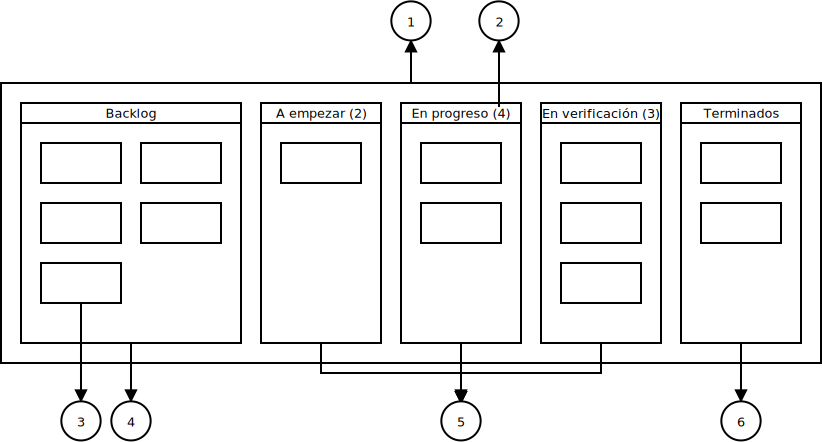
\includegraphics[width=0.85\linewidth]{5-Cuerpo/Chapter2/TablonKanban.png}
    \caption{Ejemplo de un tablón kanban}\label{fig:kanbanboard}
\end{figure}
\improvement{INSERTAR UNA IMAGEN DE UN TABLÓN KANBAN COMPLETO}

Como se puede observar en la figura~\ref{fig:kanbanboard}, muchos de los elementos visibles ya
habían sido referenciados anteriormente; sin embargo, se procederá a dar una
explicación detallada de lo que representan y qué rol cumplen:

\begin{itemize}
    \item \textbf{Tablón}: % kanban board
    Como núcleo de la visualización del proceso está el tablón kanban (nótese la
    diferencia en la capitalización del nombre). Dichos tablones contienen las
    listas de tareas a realizar y permiten observar el flujo de trabajo del
    equipo a través de columnas y cartas. Cada grupo deberá especificar su
    propio tablón kanban en función de su proceso de desarrollo y es a través de
    éste que se podrán calcular las métricas, encontrar los ciclos de
    retroalimentación y determinar qué se debe mejorar para maximizar la
    eficiencia. En la figura~\ref{fig:kanbanboard} está representado por el
    elemento $1$.

    \item \textbf{Listas o Columnas}:
    Para poder visualizar correctamente el flujo de trabajo dentro del tablón
    kanban se hacen uso de listas de tareas o columnas. Dichos elementos
    representarán los pasos que debe seguir una tarea para pasar por todo el
    flujo desde que se plantea como labor hasta que se finaliza. En el método se
    dice que las tareas son \emph{tiradas} (\emph{pulled} en inglés) a la
    siguiente lista una vez que se cumplen las condiciones de finalización de la
    columna en la que se encuentra. Entre los tipos de columnas que se pueden
    encontrar están:
    \begin{itemize}
        \item \textbf{Backlog}: Contiene la lista de tareas que se plantean
        realizar, pero aún no se han empezado o que pueden terminar siendo
        descartados. Éstas son las ideas de lo que se quiere desarrollar, pero
        que aún no se han materializado en labor. Dichos elementos deberán estar
        enfocados a contribuir con los objetivos del producto a implementar. En
        la figura~\ref{fig:kanbanboard} está representada por el elemento $4$.
        \item \textbf{Listas intermedias}: El tablón kanban, al depender mucho
        proceso del equipo y no poder ser estandarizado, hará uso también de
        distintas columnas intermedias entre el \emph{backlog} y la columna de
        tareas finalizadas. Dichas listas serán representativas del flujo de
        trabajo que sigue el grupo como tal para desarrollar el proyecto.
        Tipicamente se pueden encontrar columnas como: \emph{a diseñar}, \emph{a
        empezar}, \emph{en progreso}, \emph{en verificación}, entre otras. En la
        figura~\ref{fig:kanbanboard} están representadas por el elemento $5$.
        \item \textbf{Terminado}: Contiene la lista de tareas que se han dado
        por finalizadas en su totalidad. Esta columna es la última del tablón
        para el equipo y aquí es donde estarán todas las tareas completadas una
        vez que han pasado por todo el flujo de desarrollo. En la
        figura~\ref{fig:kanbanboard} está representada por el elemento $6$.
    \end{itemize}

    \item \textbf{WiP}: Con el fin de aplicar las prácticas de limitación y
    manejo del flujo de trabajo, a cada columna se le asigna un límite de tareas
    que puede contener en un determinado momento. Si dicha lista llega a su
    límite, no se podrán traer tareas a ella hasta que se liberé de los labores
    que contiene. Normalmente dicho límite se escribe al lado del nombre de su
    respectiva columna. En la figura~\ref{fig:kanbanboard} está representado por el
    elemento $2$.

    \item \textbf{Cartas}:
    Así como el tablón kanban contiene listas de trabajo, dichas columnas
    también contienen unos elementos conocidos como \emph{cartas}. Éstas
    representan las actividades y trabajos a realizar con el fin de avanzar con
    proyecto, siempre teniendo en cuenta que dichos elementos deben aumentar el
    valor del producto y tienen que ser significados para su finalización. En la
    figura~\ref{fig:kanbanboard} están representadas por el elemento $3$.
\end{itemize}

\subsection{Métricas de flujo}
Para finalizar con el contenido teórico del método, se hablarán de las distintas
métricas que se utilizan para determinar la eficiencia del proceso y los
elementos a mejorar según la metodología Kanban. Daniel S. Vacanti define
en~\cite{Daniel2022} la siguiente lista de medidas:\improvement{Preguntar si
esta referencia se debe escribir así}

\begin{itemize}
    \item \textbf{Trabajo en progreso}: Es el número de elementos o cartas de
    trabajo iniciados pero no finalizados.
    \item \textbf{Rendimiento}: Es el número de elementos de trabajo finalizados
    por unidad de tiempo.
    \item \textbf{Edad del elemento de trabajo}: Es el tiempo transcurrido desde
    que se inició el trabajo hasta el momento actual.
    \item \textbf{Tiempo de ciclo}: Es la cantidad de tiempo transcurrido desde
    que se inicia un trabajo y se termina.
\end{itemize}

\subsection{Justificación de la metodología}

Una vez conocidos los aspectos teóricos de la metodología, se puede proceder con
la justificación de su elección. Como tal, al ser un proyecto planteado por el
propio autor, se espera mucha variabilidad a la hora de definir y plantear los
distintos objetivos, requisitos y supuestos del producto a desarrollar. Es por
esta razón que se considera necesaria la utilización de una metodología ágil que
permita adaptarse a los cambios inesperados que irán surgiendo. Además, esta
ventaja está reforzada por el hecho de que el autor no dispone de un horario de
trabajo muy flexible y que existirá la necesidad de formarse en distintas
tecnologías parcialmente o totalmente desconocidas.

Se puede decir, entonces, que el proyecto se caracteriza por su alto nivel de
desconocimiento en cuanto a estimaciones, conocimiento y alcance general y su
necesidad por un proceso iterativo y ágil. Por tanto, la metodología Kanban se
plantea como la herramienta perfecta para su desarrollo.

% -----------------------------------------------------------------------------

\subsection{Adaptación de la metodología}\label{subsec:kanban_adaptacion}

Conociendo la justificación, ahora surge una pregunta muy importante de cara a
la implementación de la metodología: ¿cómo se adaptará para la gestión y
realización del proyecto?

Haciendo referencia a la práctica de \emph{definición y visualización del flujo
de trabajo}, Kanban recomienda el uso de un tablón con el que se pueda
interactuar físicamente, pero existen múltiples servicios webs que permiten la
creación y gestión de equivalentes online. Ambas formas de presentar el
tablón tienen sus ventajas y desventajas; sin embargo, debido a que para este proyecto es
necesario el acceso asíncrono y virtual a las herramientas de la metodología, se
plantea hacer uso de un servicio conectado a internet desarrollado
específicamente para la gestión de tablones: \emph{Trello}.

La especificación de cómo se adapta el proceso de desarrollo a esta nueva
herramienta y a la metodología Kanban se realizará haciendo uso de las
recomendaciones encontradas en~\cite{Brechner2015-dv} y se explicará en función
de las prácticas del método con las que cumplen.

\subsubsection{Trello como herramienta de gestión}

\change[inline]{Uno de los artefactos es el tablón como tal. Aquí se define Trello como tablón online/virtual}
\change[inline]{Definición de Trello y un poco de transfondo}
\change[inline]{
Trello is a collaboration tool that organizes your projects into boards. In one
glance, Trello tells you what's being worked on, who's working on what, and
where something is in a process.
Imagine a white board, filled with lists of sticky notes, with each note as a
task for you and your team. Now imagine that each of those sticky notes has
photos, attachments from other data sources like BitBucket or Salesforce,
documents, and a place to comment and collaborate with your teammates.
Now imagine that you can take that whiteboard anywhere you go on your
smartphone, and can access it from any computer through the web. That's Trello!(\cite{Trello2021})
}

\subsubsection{Aplicando las prácticas de Kanban}
\begin{itemize}
    \item \textbf{Definir y visualizar el flujo de trabajo}:
    \change[inline]{Define aquí el tablón, las listas, las etiquetas y el formato de
    las cartas}
    \paragraph{Tablón y columnas}

    \urgent[inline]{INSERTAR CAPTURA DEL TABLÓN DE TRELLO}

    \begin{itemize}
        \item \textbf{Backlog}: La columna que contendrá la lista de tareas e ideas
       espera de ser empezadas en la iteración.
        \item \textbf{To Do}: Del inglés \emph{a hacer}, contiene la lista de
        tareas cuya labor ha sido empezada en la iteración.
        \item \textbf{Doing}: Del inglés \emph{en progreso}, contiene la lista de
        tareas cuya labor se está realizando en la iteración.
        \item \textbf{Testing}: Del inglés \emph{en verificación}, contiene la lista de
        tareas cuya labor se ha finalizado pero todavía se está determinando si
        cumplen con las condiciones de finalización para pasar a la lista de tareas
        terminadas.
        \item \textbf{Done}: Del inglés \emph{terminado}, contiene la lista de
        tareas cuya labor se ha dado por terminada y que están en espera de ser
        discutidas en la reunión de fin de iteración.
        \item \textbf{Approved}: Del inglés \emph{aprobado}, contiene la lista de
        tareas discutidas y cuya realización ha sido aceptada como adecuada para la
        finalización del proyecto.
    \end{itemize}

    \paragraph{Cartas}

    \urgent[inline]{HAZ REFERENCIA A LA VERSIÓN RESUMIDA DE LA CARTA QUE SE VE EN EL TABLÓN}
    \urgent[inline]{AÑADE UNA CAPTURA DE LO QUE SE VE EN LA CARTA UNA VEZ SE EXTIENDE}

    \begin{itemize}
        \item \textbf{Iteraciones}:
        \item \textbf{Código}:
        \item \textbf{Tarea}:
        \item \textbf{Tiempo Usado}:
        \item \textbf{Descripción}:
    \end{itemize}

    \paragraph{Etiquetas}
    \urgent[inline]{LAS ETIQUETAS SON INFORMACIÓN ADICIONAL QUE PERMITE TRELLO AÑADIR A LAS CARTAS}

    \begin{itemize}
        \item \textbf{Bug}: Cuando se detecta un error y se debe arreglar
        \item \textbf{Bloqueado}: Cuando una tarea no se puede completar debido a
        otras circunstancias
        \item \textbf{Pendiente}: Abreviado de “Pendiente de Retroalimentación”.
        Indica que esta tarea debe discutirse en una reunión
        \item \textbf{No aceptada}: Indica que la tarea no ha sido aceptada para
        continuar en la siguiente iteración y debe retrabajarse, cambiarse o
        descartarse.
    \end{itemize}

    \item \textbf{Limitar y manejar el trabajo en progreso}:
    % Definir aquí los WiPs
    \urgent{DEFINE LOS WIPS DE LAS COLUMNAS}
    \begin{itemize}
        \item \textbf{Backlog}: No se le aplica un WiP.
        \item \textbf{To Do}: Primero fue 2 y ahora es 4
        \item \textbf{Doing}: Primero fue 2 y ahora es 3
        \item \textbf{Testing}: 2 (debido a que hay muchas tareas de
        documentación, no hace falta más espacio para verificar)
        \item \textbf{Done}: No se le aplica un WiP
        \item \textbf{Approved}: No se le aplica un WiP
    \end{itemize}

    \item \textbf{Hacer explícitas las políticas de proceso}:
    % Criterios de finalización aquí

    \urgent[inline]{Se comentó que hay que definir el concepto de “finalizado” para cada lista. Aquí se hace eso}
    % Qué cosas se cumplen para que una carta se mueva a la siguiente lista. Agile Project Managament With Kanban pag. 24 (set limits on chaos and Step 4: Define done)
    % Pull Criteria

    \item \textbf{Implementar ciclos de retroalimentación}:
    % Reuniones de fin de iteración y de replanificación
    \urgent[inline]{EXPLICAR CÓMO SE DETERMINA LA MEJORA DEL PROCESO DE DESARROLLO. (SE TIENEN REUNIONES DE ITERACIÓN, POR EJEMPLO)}
\end{itemize}

\section{Tareas y estimación de dedicaciones}
No se puede predecir porque usamos Kanban. Sólo conocemos las fechas finales de
entrega.
\subsection{Descripción de tareas a realizar}

\subsection{Dependencias entre tareas}

\subsection{Periodo de desarrollo de tareas}

\subsection{Estimación de dedicación a cada una de las tareas}

\subsection{Hitos de desarrollado}


\section{Análisis de riesgos y viabilidad}

% \section{Asignación de responsabilidades}

\section{Caracterización del sistema de información y del sistema de comuniaciones}

\subsection{Sistema de Información}
\subsubsection{Estructura}
Aquí debemos explicar la estructura

TFG: Directorio principal del proyecto

\begin{itemize}
    \item TFG.Proyecto:
    \begin{itemize}
        \item Memoria:
        \item Framework:
        \begin{itemize}
            \item Lenguaje:
            \item Core:
            \item CLI:
        \end{itemize}
        \item Manual:
    \end{itemize}
    \item TFG.Gestión:
    \begin{itemize}
        \item Planificación:
        \item Seguimiento:
        \item Actas:
    \end{itemize}
    \item TFG.Defensa:
\end{itemize}

\subsubsection{Formato}
\subsubsection{Denominación}
\subsubsection{Copias de seguridad}
Usamos GitHub para control de versiones y copias de seguridad

\subsection{Comunicaciones}
Reuniones
[Comunicaciones para responder dudas]
\chapter{Gestión del proyecto}\label{ch:gestion}

\section{Alcance}\label{sec:alcance}

El alcance de este proyecto incluye el trabajo necesario para diseñar,
implementar y documentar un framework de modelado y desarrollo de simulación de
sistemas dinámicos discretos basados en eventos. Dicho framework se dividirá en
tres módulos principales:
\begin{itemize}
    \item Lenguaje: Un lenguaje de modelado específico pensado para ser usado
    por usuarios que no tengan mucha experiencia en programación. Se hará uso de
    las herramientas de desarrollo de compiladores Flex y Bison para generar un
    transpilador que traduzca ficheros de este lenguaje a código Python. A
    través de él se plantea:
    \begin{itemize}
        \item Permitir la rápida implementación de este tipo de modelos a través
        de grafos de sucesos.
        \item Permitir que el programador del lenguaje se encargue sólo de
        realizar las implementaciones pertinentes al sistema de simulación que
        desee desarrollar:
        \begin{itemize}
            \item Especificación de las variables globales, variables de
            entrada, contadores estadísticos y medidas de rendimiento propias
            del modelo.
            \item Inclusión de eventos adicionales y sus acciones
            correspondientes.
            \item Creación y eliminación de eventos en función de tiempo y
            condiciones lógicas.
            \item Inclusión de código adicional escrito directamente en Python
            en caso de ser necesario.\urgent{Cambiar redacción}
        \end{itemize}
    \end{itemize}
    \item Núcleo: Una serie de módulos que implementarán un microframework de
    simulación de este tipo de sistemas en específico para Python, pensado para
    ser usado por programadores y para acotar la traducción del nuevo lenguaje.
    A través de él se plantea:
    \begin{itemize}
        \item Permitir que la traducción del lenguaje incluya dentro del fichero
        generado las estructuras de datos, funciones y procedimientos que tienen
        en común todos los sistemas dinámicos discretos:
        \begin{itemize}
            \item Generadores de datos aleatorios para distintos tipos de
            distribuciones.
            \item Reloj y temporizador de simulación para ejecutar los eventos.
            \item Estructura de datos para almacenar los sucesos según deben
            ocurrir en el tiempo.
            \item Las respectivas implementaciones mínimas de los dos eventos
            que siempre formarán parte de todos los modelos: “Inicio” y “Fin”.
            \item Generador de informes final que se ejecutará al finalizar la
            simulación y mostrará los resultados que se deseaban estudiar con
            ésta.
        \end{itemize}
    \end{itemize}
    \item CLI: Una interfaz de comandos por terminal que se usará para
    gestionar, configurar y ejecutar los proyectos desarrollados con este
    framework.
\end{itemize}

\subsection{Objetivos}

\subsubsection{Objetivo general}
Generar un lenguaje de modelado de simulación de sistemas dinámicos discretos
basados en eventos junto con un transpilador que lo traduzca a Python, un
microframework para acotar la traducción y un CLI para gestionar proyectos
desarrollados con este producto.

\subsubsection{Objetivos específicos}
\begin{enumerate}
    \item Diseñar un nuevo lenguaje de modelado y simulación de sistemas
    dinámicos discretos basados en eventos usando las herramientas de desarrollo
    de procesadores de lenguaje Flex y Bison.
    \item Diseñar, implementar y verificar una serie de módulos y
    funcionalidades realizadas en Python con el fin de generar un microframework
    para simular estos mismos sistemas.
    \item Implementar y verificar un transpilador que traduzca el lenguaje del
    producto a Python usando las características del objetivo anterior.
    \item Diseñar, implementar y verificar una serie de operaciones accesibles
    desde una CLI de cara a ser usadas para la gestión, configuración y
    ejecución parametrizada de simulaciones realizadas con el producto.
    \item Implementar distintas técnicas de análisis de salidas, experimentación
    y optimización de modelos dentro del núcleo del framework.
    \item Desarrollar un manual de usuario que contendrá toda la documentación
    necesaria para hacer uso del framework.
\end{enumerate}

\subsection{Requisitos}
El requisito base principal del proyecto consiste en cumplir con un tiempo de
dedicación total máximo de 300 horas. Sin embargo, se pueden listar otros
requisitos específicos:

\subsubsection{Caracterización de la memoria}
Debe ser bien citado y referenciado para evitar el plagio
Se debe utilizar una metodología de citas.
Apartado de calidad

\subsubsection{Caracterización del framework}
Un lenguaje verificado que no pete a la primera
El resultado son métricas en un dataframe (o varios si harás lo de validación)
Cumplir con la línea base de calidad definida en el apartado (...)

\subsubsection{Caracterización del manual}
Utilizar referencias a recursos ajenas

\subsubsection{Licencia del producto}

\subsection{Entregables}

\begin{itemize}
    \item Memoria: \change{Relacionados con el objeto de proyecto en sí}
    \item Framework:\change{Relacionados con el objeto de proyecto en sí}
    \item Manual: \change{Relacionados con el objeto de proyecto en sí}
    \item Planificación: \change{Relacionados con la Planificación y Gestión del
    Proyecto}
    \item Seguimiento y Control: \change{Relacionados con la Planificación y Gestión del
    Proyecto}
    \item Actas: \change{Relacionados con la Planificación y Gestión del
    Proyecto}
\end{itemize}

\subsection{Exclusiones}

Mi proyecto devolverá los datos en un sólo formato, no devolveré más tipos de
ficheros para darle gusto al usuario.

\subsection{Supuestos}

\urgent[inline]{}

\subsection{EDT}

\begin{figure}[H]
    \centering
    \includegraphics[width=\textwidth]{5-Cuerpo/Chapter1/EDT.png}
    \caption{Esquema de Descomposición de Trabajo del Proyecto}
    \label{fig:EDT}
\end{figure}
\section{Metodología}\label{sec:metodologia}

A la hora de gestionar un proyecto, es recomendable definir una metodología de
trabajo, seguimiento y control con el fin de asegurar el correcto cumplimiento y
finalización de su lista de requisitos y objetivos. Tras investigar y plantear
distintas alternativas, se ha escogido la metodología Kanban para desarrollar
este proyecto.

El método Kanban como tal es útil si se desea:
\begin{itemize}
    \item Iniciar un proyecto de manera ágil, rápida, de coste nulo y bajo riesgo. % Getting off to a low-risk, zero-cost, agile, fast start.
    \item Analizar y mejorar el proceso de trabajo ya existente. % Pinning down existing workflows and spotting glaring errors.
    \item Controlar múltiples grupos de tareas. % Controlling multiple pieces of unconnected work.
    \item Asegurar que el número de tareas en ejecución están dentro de un nivel aceptable. % Keeping the numbers of jobs in play down to an acceptable level.
    \item Cambiar a una mentalidad de desarrollo ágil. % Getting the team into an agile way of thinking.
\end{itemize}

Esta sección, por tanto, estará dedicada a explicar los conceptos e ideas
necesarias de cara a justificar la razón por la cual se ha escogido este método
de trabajo. Además, es necesario mencionar que esta información será resumida
principalmente de~\cite{Cole2015-fd} y~\cite{Stellman2014-qr}, siendo éstas las
referencias recomendadas en caso de desear más detalles al respecto.
\subsection{Definición}

El método Kanban tiene sus orígenes en las fábricas de coches de Toyota a manos
de Taiichi Ohno. Fue creado como un simple sistema de planificación y
administración de trabajo e inventario de cada fase de producción. Sin embargo,
fue David J. Anderson quien definió y adaptó esta metodología para el uso en
ingeniería y desarrollo de software.

Es necesario mencionar que, contrario a lo que se piensa normalmente, Kanban es
una metodología ágil de mejora de procesos y no un framework de administración
de proyectos. Y así como muchos métodos de este tipo, se caracteriza
principalmente por ser evolutivo e iterativo en el tiempo.

Asimismo, Kanban comparte la misma ideología de trabajo con el método Lean hasta
tal punto que se considera que es una especialización de esta última. Aplicando
los principios y valores de este proceso, Kanban se centra en eliminar los
desperdicios de tiempo y recursos que el equipo tiene. Por lo tanto, este
proceso de mejora pide a los equipos de desarrollo empezar con una metodología
ya existente para poder perfeccionarla gradualmente en el tiempo a través de la
experimentación, el cálculo de distintas métricas de rendimiendo y la
confirmación de resultados positivos según dichas medidas.

Todo equipo cuenta con un sistema para la implementación de código, ya sea que
se siga una metodología formal como Scrum o que se disponga de una serie de
reglas no definidas o reconocidas explícitamente. Como consecuencia de esto, lo
único que se necesita para empezar a utilizar Kanban es identificar el proceso
de desarrollo actual para poder formalizarlo y adaptarlo a esta metodología.

Por tanto, aunque Kanban no es un sistema de gestión de proyectos, es posible
hacer uso de éste para ello al tener como principal objetivo aumentar la
predictabilidad del flujo de trabajo y así mejorar la planificación del proyecto
como tal.

\subsection{Principios de Kanban}
Al ser una especialización del método Lean, se tiene una serie de principios
directores en esta metodología. Especificamente se pueden listar los siguientes
tres:
\begin{itemize}
    \item \textbf{Empieza con lo que se hace actualmente}: %Start with what you do now
    Como se había mencionado anteriormente, el método Kanban pide requiere de un
    proceso o metodología inicial. Es a través del análisis y la comprensión de
    dicho proceso que Kanban permite perfeccionarlo iterativamente. Pero como
    consecuencia de esto, no es posible aplicar Kanban adecuadamente si se
    desconoce la metodología que usa el equipo de desarrollo.

    \item \textbf{Comprométete al cambio evolutivo e incremental}: %Agree to pursue incremental, evolutionary change
    Aunque parezca muy repetitivo, es necesario volver a mencionar que el
    objetivo de Kanban es la mejora gradual del sistema. A eso se refiere el
    cambio evolutivo e incremental y es por eso que el método pide calcular
    métricas de control. Es a través de estas medidas que se llegan a conocer
    las partes mejores del proceso de desarrollo.

    \item \textbf{Respeta el proceso, los roles, las responsabilidades y títulos
    actuales}: %Respect the current process, roles, responsibilities and titles
    Cuando el equipo de trabajo dedica tiempo a medir el rendimiento del
    sistema, es posible encontrar ciclos de retroalimentación que contienen
    información importante para la mejora evolutiva del proceso. Sin embargo,
    para poder aplicar dicha información es necesario conocer cómo se aplica
    ésta a cada rol del equipo. Por esta razón Kanban considera relevante
    respetar las responsabilidades y roles asociadas a cada miembro del grupo.
\end{itemize}

\subsection{Prácticas de Kanban}

El método Kanban, además, define explícitamente una serie de prácticas a llevar
a cabo con el fin de aplicar correctamente la mejora de procesos que éste
permite. Sin embargo, no es necesario hacer uso de todas estas en su totalidad
al iniciar con el método. Kanban tiene específicamente los siguientes seis principios:

\begin{itemize}
    \item \textbf{Definir y visualizar el flujo de trabajo}: %Define and Visualise Workflow
    Con el fin de familiarizarse más con el proceso de trabajo, Kanban pide
    hacer uso de representaciones visuales de éste a través de tablones, listas
    de trabajo y elementos de trabajo. La combinación de dichos componentes
    permite definir el flujo de trabajo en su totalidad de una manera fácilmente
    entendible. En Kanban, visualizar significa anotar exactamente lo que hace
    el equipo sin embellecer los detalles con el fin de observar el sistema en
    su totalidad.

    \item \textbf{Limitar el trabajo en progreso}: %Limit work-in-progress
    En el método Kanban los distintos trabajos a realizar en el proceso de
    desarrollo tienen un límite de tareas en ejecución en un determinado
    momento. La justificación que se le da a este principio recae en el hecho de
    que realizar múltiples labores a la vez reduce la eficiencia del equipo. A
    dicho límite se le conoce como \emph{WiP} (de sus siglas en inglés
    \emph{Work-in-Progress}) o \emph{Trabajo en Progreso}.

    \item \textbf{Manejar el flujo de trabajo}: %Manage the flow of work
    Una vez definido el flujo de trabajo, el objetivo será conseguir una rápida
    y suave transición entre los distintos grupos de tareas, desde la lista de
    trabajo a empezar hasta dar por finalizada la labor. Si se consigue esta
    velocidad de flujo, se dice que se está operando con la eficiencia óptima y
    es en este momento que se crea el máximo valor laboral en el menor tiempo
    posible. A medida que el equipo desarrolla, se van encontrando los cuellos
    de botella y ajustando los límites de trabajo.

    \item \textbf{Hacer explícitas las políticas de proceso}: %Make the process explicit
    Para poder obtener un flujo de trabajo óptimo, además, es necesario definir
    los objetivos que se deben cumplir para dar por terminada una serie de
    tareas con el fin de determinar cuándo se avanza de estado. Dichas
    condiciones de finalización, sin embargo, siempre irán ligadas al tipo de
    proceso que se está utilizando y, por tanto, deberán ser discutidas y
    especificadas por el equipo.

    \item \textbf{Implementar ciclos de retroalimentación}: %Implement Feedback Loops
    Como se había mencionado anteriormente, los ciclos de retroalimentación
    permiten identificar la información necesaria para aplicar mejoras en el
    proceso de desarrollo. Kanban define dichos ciclos como la combinación de
    limitaciones que permiten dar a conocer los puntos débiles del equipo y su
    correcta implementación requiere de experimentación y análisis del
    rendimiento general del sistema.

    \item \textbf{Mejorar colaborativamente}: %Improve collaboratively
    Una vez que Kanban ya está implementado y el foco de atención recae en el
    flujo de trabajo, el carácter de mejora incremental del método vuelve a
    salir a la luz. Es a través de la discusión, análisis y puesta en marcha de
    nuevas ideas que el equipo puede encontrar bloqueos en el proceso y
    adaptarse a cambios rápidamente.
\end{itemize}

\subsection{Herramientas de Kanban}

Para poder hacer uso de los principios y aplicar correctamente las prácticas del
método, existe una serie de herramientas y artefactos comunes dentro de la
metodología Kanban.

\begin{figure}[H]
    \centering
    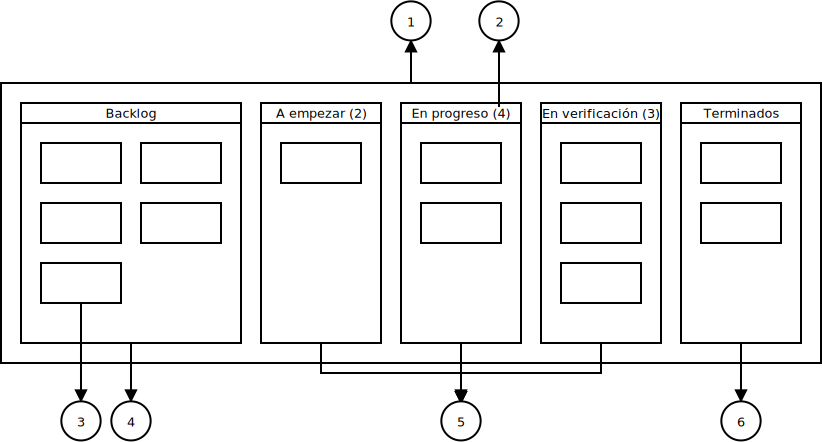
\includegraphics[width=0.85\linewidth]{5-Cuerpo/Chapter2/TablonKanban.png}
    \caption{Ejemplo de un tablón kanban}\label{fig:kanbanboard}
\end{figure}
\improvement{INSERTAR UNA IMAGEN DE UN TABLÓN KANBAN COMPLETO}

Como se puede observar en la figura~\ref{fig:kanbanboard}, muchos de los elementos visibles ya
habían sido referenciados anteriormente; sin embargo, se procederá a dar una
explicación detallada de lo que representan y qué rol cumplen:

\begin{itemize}
    \item \textbf{Tablón}: % kanban board
    Como núcleo de la visualización del proceso está el tablón kanban (nótese la
    diferencia en la capitalización del nombre). Dichos tablones contienen las
    listas de tareas a realizar y permiten observar el flujo de trabajo del
    equipo a través de columnas y cartas. Cada grupo deberá especificar su
    propio tablón kanban en función de su proceso de desarrollo y es a través de
    éste que se podrán calcular las métricas, encontrar los ciclos de
    retroalimentación y determinar qué se debe mejorar para maximizar la
    eficiencia. En la figura~\ref{fig:kanbanboard} está representado por el
    elemento $1$.

    \item \textbf{Listas o Columnas}:
    Para poder visualizar correctamente el flujo de trabajo dentro del tablón
    kanban se hacen uso de listas de tareas o columnas. Dichos elementos
    representarán los pasos que debe seguir una tarea para pasar por todo el
    flujo desde que se plantea como labor hasta que se finaliza. En el método se
    dice que las tareas son \emph{tiradas} (\emph{pulled} en inglés) a la
    siguiente lista una vez que se cumplen las condiciones de finalización de la
    columna en la que se encuentra. Entre los tipos de columnas que se pueden
    encontrar están:
    \begin{itemize}
        \item \textbf{Backlog}: Contiene la lista de tareas que se plantean
        realizar, pero aún no se han empezado o que pueden terminar siendo
        descartados. Éstas son las ideas de lo que se quiere desarrollar, pero
        que aún no se han materializado en labor. Dichos elementos deberán estar
        enfocados a contribuir con los objetivos del producto a implementar. En
        la figura~\ref{fig:kanbanboard} está representada por el elemento $4$.
        \item \textbf{Listas intermedias}: El tablón kanban, al depender mucho
        proceso del equipo y no poder ser estandarizado, hará uso también de
        distintas columnas intermedias entre el \emph{backlog} y la columna de
        tareas finalizadas. Dichas listas serán representativas del flujo de
        trabajo que sigue el grupo como tal para desarrollar el proyecto.
        Tipicamente se pueden encontrar columnas como: \emph{a diseñar}, \emph{a
        empezar}, \emph{en progreso}, \emph{en verificación}, entre otras. En la
        figura~\ref{fig:kanbanboard} están representadas por el elemento $5$.
        \item \textbf{Terminado}: Contiene la lista de tareas que se han dado
        por finalizadas en su totalidad. Esta columna es la última del tablón
        para el equipo y aquí es donde estarán todas las tareas completadas una
        vez que han pasado por todo el flujo de desarrollo. En la
        figura~\ref{fig:kanbanboard} está representada por el elemento $6$.
    \end{itemize}

    \item \textbf{WiP}: Con el fin de aplicar las prácticas de limitación y
    manejo del flujo de trabajo, a cada columna se le asigna un límite de tareas
    que puede contener en un determinado momento. Si dicha lista llega a su
    límite, no se podrán traer tareas a ella hasta que se liberé de los labores
    que contiene. Normalmente dicho límite se escribe al lado del nombre de su
    respectiva columna. En la figura~\ref{fig:kanbanboard} está representado por el
    elemento $2$.

    \item \textbf{Cartas}:
    Así como el tablón kanban contiene listas de trabajo, dichas columnas
    también contienen unos elementos conocidos como \emph{cartas}. Éstas
    representan las actividades y trabajos a realizar con el fin de avanzar con
    proyecto, siempre teniendo en cuenta que dichos elementos deben aumentar el
    valor del producto y tienen que ser significados para su finalización. En la
    figura~\ref{fig:kanbanboard} están representadas por el elemento $3$.
\end{itemize}

\subsection{Métricas de flujo}
Para finalizar con el contenido teórico del método, se hablarán de las distintas
métricas que se utilizan para determinar la eficiencia del proceso y los
elementos a mejorar según la metodología Kanban. Daniel S. Vacanti define
en~\cite{Daniel2022} la siguiente lista de medidas:\improvement{Preguntar si
esta referencia se debe escribir así}

\begin{itemize}
    \item \textbf{Trabajo en progreso}: Es el número de elementos o cartas de
    trabajo iniciados pero no finalizados.
    \item \textbf{Rendimiento}: Es el número de elementos de trabajo finalizados
    por unidad de tiempo.
    \item \textbf{Edad del elemento de trabajo}: Es el tiempo transcurrido desde
    que se inició el trabajo hasta el momento actual.
    \item \textbf{Tiempo de ciclo}: Es la cantidad de tiempo transcurrido desde
    que se inicia un trabajo y se termina.
\end{itemize}

\subsection{Justificación de la metodología}

Una vez conocidos los aspectos teóricos de la metodología, se puede proceder con
la justificación de su elección. Como tal, al ser un proyecto planteado por el
propio autor, se espera mucha variabilidad a la hora de definir y plantear los
distintos objetivos, requisitos y supuestos del producto a desarrollar. Es por
esta razón que se considera necesaria la utilización de una metodología ágil que
permita adaptarse a los cambios inesperados que irán surgiendo. Además, esta
ventaja está reforzada por el hecho de que el autor no dispone de un horario de
trabajo muy flexible y que existirá la necesidad de formarse en distintas
tecnologías parcialmente o totalmente desconocidas.

Se puede decir, entonces, que el proyecto se caracteriza por su alto nivel de
desconocimiento en cuanto a estimaciones, conocimiento y alcance general y su
necesidad por un proceso iterativo y ágil. Por tanto, la metodología Kanban se
plantea como la herramienta perfecta para su desarrollo.

% -----------------------------------------------------------------------------

\subsection{Adaptación de la metodología}\label{subsec:kanban_adaptacion}

Conociendo la justificación, ahora surge una pregunta muy importante de cara a
la implementación de la metodología: ¿cómo se adaptará para la gestión y
realización del proyecto?

Haciendo referencia a la práctica de \emph{definición y visualización del flujo
de trabajo}, Kanban recomienda el uso de un tablón con el que se pueda
interactuar físicamente, pero existen múltiples servicios webs que permiten la
creación y gestión de equivalentes online. Ambas formas de presentar el
tablón tienen sus ventajas y desventajas; sin embargo, debido a que para este proyecto es
necesario el acceso asíncrono y virtual a las herramientas de la metodología, se
plantea hacer uso de un servicio conectado a internet desarrollado
específicamente para la gestión de tablones: \emph{Trello}.

La especificación de cómo se adapta el proceso de desarrollo a esta nueva
herramienta y a la metodología Kanban se realizará haciendo uso de las
recomendaciones encontradas en~\cite{Brechner2015-dv} y se explicará en función
de las prácticas del método con las que cumplen.

\subsubsection{Trello como herramienta de gestión}

\change[inline]{Uno de los artefactos es el tablón como tal. Aquí se define Trello como tablón online/virtual}
\change[inline]{Definición de Trello y un poco de transfondo}
\change[inline]{
Trello is a collaboration tool that organizes your projects into boards. In one
glance, Trello tells you what's being worked on, who's working on what, and
where something is in a process.
Imagine a white board, filled with lists of sticky notes, with each note as a
task for you and your team. Now imagine that each of those sticky notes has
photos, attachments from other data sources like BitBucket or Salesforce,
documents, and a place to comment and collaborate with your teammates.
Now imagine that you can take that whiteboard anywhere you go on your
smartphone, and can access it from any computer through the web. That's Trello!(\cite{Trello2021})
}

\subsubsection{Aplicando las prácticas de Kanban}
\begin{itemize}
    \item \textbf{Definir y visualizar el flujo de trabajo}:
    \change[inline]{Define aquí el tablón, las listas, las etiquetas y el formato de
    las cartas}
    \paragraph{Tablón y columnas}

    \urgent[inline]{INSERTAR CAPTURA DEL TABLÓN DE TRELLO}

    \begin{itemize}
        \item \textbf{Backlog}: La columna que contendrá la lista de tareas e ideas
       espera de ser empezadas en la iteración.
        \item \textbf{To Do}: Del inglés \emph{a hacer}, contiene la lista de
        tareas cuya labor ha sido empezada en la iteración.
        \item \textbf{Doing}: Del inglés \emph{en progreso}, contiene la lista de
        tareas cuya labor se está realizando en la iteración.
        \item \textbf{Testing}: Del inglés \emph{en verificación}, contiene la lista de
        tareas cuya labor se ha finalizado pero todavía se está determinando si
        cumplen con las condiciones de finalización para pasar a la lista de tareas
        terminadas.
        \item \textbf{Done}: Del inglés \emph{terminado}, contiene la lista de
        tareas cuya labor se ha dado por terminada y que están en espera de ser
        discutidas en la reunión de fin de iteración.
        \item \textbf{Approved}: Del inglés \emph{aprobado}, contiene la lista de
        tareas discutidas y cuya realización ha sido aceptada como adecuada para la
        finalización del proyecto.
    \end{itemize}

    \paragraph{Cartas}

    \urgent[inline]{HAZ REFERENCIA A LA VERSIÓN RESUMIDA DE LA CARTA QUE SE VE EN EL TABLÓN}
    \urgent[inline]{AÑADE UNA CAPTURA DE LO QUE SE VE EN LA CARTA UNA VEZ SE EXTIENDE}

    \begin{itemize}
        \item \textbf{Iteraciones}:
        \item \textbf{Código}:
        \item \textbf{Tarea}:
        \item \textbf{Tiempo Usado}:
        \item \textbf{Descripción}:
    \end{itemize}

    \paragraph{Etiquetas}
    \urgent[inline]{LAS ETIQUETAS SON INFORMACIÓN ADICIONAL QUE PERMITE TRELLO AÑADIR A LAS CARTAS}

    \begin{itemize}
        \item \textbf{Bug}: Cuando se detecta un error y se debe arreglar
        \item \textbf{Bloqueado}: Cuando una tarea no se puede completar debido a
        otras circunstancias
        \item \textbf{Pendiente}: Abreviado de “Pendiente de Retroalimentación”.
        Indica que esta tarea debe discutirse en una reunión
        \item \textbf{No aceptada}: Indica que la tarea no ha sido aceptada para
        continuar en la siguiente iteración y debe retrabajarse, cambiarse o
        descartarse.
    \end{itemize}

    \item \textbf{Limitar y manejar el trabajo en progreso}:
    % Definir aquí los WiPs
    \urgent{DEFINE LOS WIPS DE LAS COLUMNAS}
    \begin{itemize}
        \item \textbf{Backlog}: No se le aplica un WiP.
        \item \textbf{To Do}: Primero fue 2 y ahora es 4
        \item \textbf{Doing}: Primero fue 2 y ahora es 3
        \item \textbf{Testing}: 2 (debido a que hay muchas tareas de
        documentación, no hace falta más espacio para verificar)
        \item \textbf{Done}: No se le aplica un WiP
        \item \textbf{Approved}: No se le aplica un WiP
    \end{itemize}

    \item \textbf{Hacer explícitas las políticas de proceso}:
    % Criterios de finalización aquí

    \urgent[inline]{Se comentó que hay que definir el concepto de “finalizado” para cada lista. Aquí se hace eso}
    % Qué cosas se cumplen para que una carta se mueva a la siguiente lista. Agile Project Managament With Kanban pag. 24 (set limits on chaos and Step 4: Define done)
    % Pull Criteria

    \item \textbf{Implementar ciclos de retroalimentación}:
    % Reuniones de fin de iteración y de replanificación
    \urgent[inline]{EXPLICAR CÓMO SE DETERMINA LA MEJORA DEL PROCESO DE DESARROLLO. (SE TIENEN REUNIONES DE ITERACIÓN, POR EJEMPLO)}
\end{itemize}
\section{Tareas y estimación de dedicaciones}\label{sec:tareas}
\change[inline]{No se puede predecir porque usamos Kanban. Sólo conocemos las fechas finales de
entrega.}



% -----------------------------------------------------------------------------


\subsection{Descripción de tareas a realizar}\label{subsec:tareas-descripcion}

\subsubsection{Gestión}
\paragraph{Planificación}
\begin{enumerate}
    \item Definición de la metodología de gestión.
    \item Generación de la planificación inicial.
    \item Automatización de herramientas de gestión con Trello.
    \item Cambios y actualizaciones de la planificación.
\end{enumerate}
\paragraph{Seguimiento y Control}
\begin{enumerate}
    \item Recogida de información sobre el desarrollo del proyecto
    \item Contraste de la información de seguimiento con los planes, identificación de desviaciones significativas y actuación ante riesgos emergentes.
    % \item Aseguramiento de las condiciones para el éxito del proyecto.
    \item Preparación de documentos de cara a la próxima reunión.
    \item Reuniones de fin de iteración
\end{enumerate}

\subsubsection{Formación e Investigación}
\begin{enumerate}
    \item Investigación y formación sobre la metodología Kanban.
    \item Profundización sobre conceptos de simulación de sistemas.
    \item Profundización sobre conceptos de compilación.
    \item Investigación y formación sobre herramientas de desarrollo de CLIs.
    \item Investigación y formación sobre generación de paquetes instalables
    para Python.
    \item Investigación y formación sobre funciones de alto nivel y paquetes
    relacionados de Python.
    \item Investigación sobre lenguajes de modelado y simulación.
    \item Investigación sobre antecedentes del proyecto.
    \item Exploración de alternativas al módulo de lenguaje.
\end{enumerate}

\subsubsection{Producto}
\paragraph{Memoria}
\begin{enumerate}
    \item Diseño y preparación de la estructura
    % \item Configuración del preámbulo %(Igual va en IyP)
    \item Redacción del resumen %(Resumen ejecutivo junto a las palabras clave)
    \item Redacción de la introducción %(Vamos a poner aquí como mucho dos página)
    \item Redactar contexto %(Aquí explicamos más a fondo el problema)
    \item Redacción de la gestión del proyecto %(Generamos la planificación y luego ponemos el seguimiento aquí mismo)
    \item Redacción del marco teórico %(Conceptos teóricos necesarios para entender el proyecto)
    \item Redacción del desarrollo %(El propio desarrollo del producto principal)
    % \item Redacción del apartado de pruebas %(Aquí pondré las pruebas que haré)
    \item Redacción de conclusiones %(Qué puedo sacar de esto, qué trabajo futuro surge de esto)
    \item Preparación e inclusión de referencias bibliográficas %(Cuidado con bibtex)
    \item Redacción de anexos %(Aquí cualquier cosa que desee añadir, actas...)
    \item Validación y corrección de los índices %(A veces fallan estos)
    \item Maquetación y diseño de la memoria %(Esto es literalmente la configuración del preámbulo)
\end{enumerate}
\paragraph{Framework}
\begin{itemize}
    \item \textbf{Lenguaje:}
    \begin{enumerate}
        \item Diseño del léxico del lenguaje.
        \item Diseño de la sintaxis del lenguaje.
        \item Diseño de la semántica del lenguaje.
        \item Diseño de módulos de cara a la implementación del lenguaje.
        \item Implementación del analizador léxico.
        \item Implementación del analizador sintáctico.
        \item Implementación de la tabla de símbolos.
        \item Implementación del análisis semántico.
        \item Documentación de los ficheros del lenguaje.
        \item Pruebas y verificación del lenguaje.
    \end{enumerate}
    \item \textbf{Núcleo:}
    \begin{enumerate}
        \item Diseño de los módulos y paquetes del núcleo.
        % Cosas en común entre todos los modelos de simulación:
        \item Implementación de la estructura de datos para almacenar eventos.
        \item Implementación del reloj y el proceso de temporización de sucesos.
        \item Implementaciones de los procesos de inicialización y finalización.
        \item Implementación del generador de informes final.
        \item Implementación de distintos generadores de datos aleatorios.
        % Cosas variables para cada modelo de simulación:
        \item Implementación de la inicialización de las variables globales,
        variables de entrada, contadores estadísticos y medidas de rendimiento
        para cualquier modelo.
        \item Implementación de la inclusión de nuevos tipos de eventos y sus
        funciones de ejecución correspondientes.
        \item Implementación de distintas estrategias de generación y
        eliminación de eventos dentro de la lista de sucesos.
        \item Implementación de la especificación de una función de parada
        definida por el usuario.
        % Funcionalidad de calidad:
        \item Implementación de la funcionalidad de configuración de la simulación.
        \item Documentación de los ficheros del núcleo.
        \item Pruebas y verificación del núcleo.
    \end{enumerate}
    \item \textbf{CLI:}
    \begin{enumerate}
        \item Diseño de las funcionalidades de la CLI.
        \item Implementación del generador de proyectos.
        \item Implementación del gestor de configuraciones del proyecto.
        \item Implementación del lanzador de modelos de simulación.
        \item Documentación de los ficheros de la CLI.
        \item Pruebas y verificación de la CLI.
    \end{enumerate}
\end{itemize}

\paragraph{Manual}
\begin{enumerate}
    \item Diseño y preparación de la estructura
    % \item Configuración del preámbulo %(Igual va en IyP)
    \item Redacción de la introducción al producto
    % \item Quickstart/Overview %(No sé si esto irá en la introducción)
    \item Especificación de dependencias y requisitos
    \item Redacción del proceso de instalación

    \item Redacción de la explicación del módulo del lenguaje
    \item Redacción de la explicación del núcleo del framework
    \item Redacción de la explicación de la CLI
    % \item Explicación de la creación, configuración y ejecución de modelos
    % (Esto es lo de la CLI)

    \item Generación de ejemplos de uso %(Necesitamos unos ejemplos prácticos, ¿no?)

    \item Preparación e inclusión de referencias bibliográficas %(Cuidado con bibtex)
    \item Redacción de anexos %(Aquí cualquier cosa que desee añadir, especificación del lenguaje, ETDS?...)
    \item Validación y corrección de los índices %(A veces fallan estos)
    \item Maquetación y diseño del manual %(Esto es literalmente la configuración del preámbulo)

\end{enumerate}

\subsubsection{Instalación y Paquetes}
\begin{enumerate}
    \item Preparación de paquetes para LaTeX.
    \item Preparación del entorno de trabajo.
    \item Instalación de paquetes para el desarrollo del lenguaje.
    \item Instalación de paquetes para el desarrollo del núcleo.
    \item Instalación de paquetes para el desarrollo de la CLI.
\end{enumerate}


% -----------------------------------------------------------------------------


% \subsection{Dependencias entre tareas}


% -----------------------------------------------------------------------------


% \subsection{Periodo de desarrollo de tareas}


% -----------------------------------------------------------------------------


\subsection{Estimación de dedicación}\label{subsec:tareas-estimacion}

\begin{table}[H]
    \centering
    \begin{tabular}{ccc}
    \textbf{Paquete} & \textbf{Nombre}                 & \textbf{Estimación (Horas)} \\
    Ge.P             & Gestión - Planificación         & 25                          \\
    Ge.S             & Gestión - Seguimiento           & 20                          \\
    FeI              & Formación e Investigación       & 50                          \\
    Pr.Me            & Proyecto - Memoria              & 50                          \\
    Pr.Fr.Le         & Proyecto - Framework - Lenguaje & 48                          \\
    Pr.Fr.Co         & Proyecto - Framework - Core     & 52                          \\
    Pr.Fr.Cli        & Proyecto - Framework - CLI      & 25                          \\
    Pr.Ma            & Proyecto - Manual               & 15                          \\
    IyP              & Instalaciones y Paquetes        & 15                          \\
    \end{tabular}
    \caption{Estimación de tiempos de dedicación por paquetes de trabajo}
    \label{tab:estimacion-paquetes}
\end{table}


% -----------------------------------------------------------------------------


% \subsection{Hitos de desarrollado}

\section{Análisis de riesgos y viabilidad}

\subsection{Métricas}

\subsection{Tabla de riesgos}
\section{Sistema de información y comunicaciones}


% -----------------------------------------------------------------------------


\subsection{Sistema de Información}

\subsubsection{Estructura}

\improvement{Aquí debemos explicar la estructura}

\textbf{TFG:} Directorio principal del proyecto. Se divide en:

\begin{itemize}
    \item \textbf{TFG.Proyecto:} Aquí residen los entregables del proyecto.
    \begin{itemize}
        \item \textbf{Memoria:} Los ficheros relacionados a la memoria
        \item \textbf{Framework:} Los ficheros relacionados al framework
        \begin{itemize}
            \item \textbf{Lenguaje:} Los ficheros relacionados al lenguaje del framework
            \item \textbf{Core:} Los ficheros relacionados al núcleo del framework
            \item \textbf{CLI:} Los ficheros relacionados al CLI del framework
            \improvement{EXISTE LA NECESIDAD DE CAMBIAR DE UN CLI A UNA GUI}
        \end{itemize}
        \item \textbf{Manual:} Los ficheros relacionados al manual
    \end{itemize}
    \item \textbf{TFG.Gestión:} Aquí residen los ficheros relacionados a la gestión del proyecto
    \begin{itemize}
        \item \textbf{Planificación:} Los ficheros relacionados a la planificación
        \item \textbf{Seguimiento:} Los ficheros relacionados al seguimiento y control
        \item \textbf{Actas:} Las actas de cada reunión realizada
    \end{itemize}
\end{itemize}

% \subsubsection{Formato}

% \subsubsection{Denominación}

\subsubsection{Copias de seguridad}
\change[inline]{Usamos GitHub para control de versiones y copias de seguridad}
\change[inline]{Todo está dividido en varios módulos y submódulos.}
\change[inline]{Los enlaces a todo están en: \url{https://github.com/brodriguez059/TFG}}
\change[inline]{Usamos Drive para generar las actas de fin de iteración}


% -----------------------------------------------------------------------------


\subsection{Comunicaciones}

\begin{itemize}
    \item (Reuniones a través de Webex)
    \item (Comunicaciones para responder dudas a través de email)
\end{itemize}
% \chapter{Marco Teórico}

\section{Simulación}\label{sec:simulacion}

%% Todavía no se ha explicado lo que es la simulación de sistemas

% Bloque simulación de sistemas

% \change[inline]{Definición de simulación}
% \change[inline]{Explicación sobre simulación de sistemas.}
% \change[inline]{¿Por qué y para qué la simulación de sistemas?}
% \change[inline]{Puedes citar a uno de tus libros aquí.}

\subsection{Definiciones}

\subsubsection{Modelo}

% \change[inline]{Haz una cita a la definición de tu profesor de simulación de
% sistemas (igual no se puede)}
% %https://normas-apa.org/referencias/citar-curso-o-material-de-clase/

% \change[inline]{Definición de modelo (Nos centraremos en modelos
% probabilísticos)}

% \change[inline]{¿Clasificación de modelos? (los modelos de simulación deben
% ser simbólicos (no tienen una relación física o analógica con el sistema real,
% sino una relación lógica))}

% \change[inline]{¿Qué significa ser dinámico?}
% \change[inline]{¿Qué significa ser discreto?}

\subsubsection{Sistema}
% \change[inline]{Definición de sistema}
% \change[inline]{Partes y conceptos de un sistema de simulación (entorno del
% sistema, entidad, atributo, actividad, estado, suceso, término endógeno,
% término exógeno, contadores estadísticos, medidas de rendimiento)}

\subsection{Ventajas e inconvenientes}
% \change[inline]{Ventajas e inconvenientes}

\subsection{Diseño basado en eventos}
% \change[inline]{Grafo de sucesos}

\subsection{Sistemas dinámicos discretos}
% \change[inline]{Partes fundamentales (en común) de los simuladores dinámicos
% discretos (lista de sucesos, temporizador de eventos, reloj...)}

\section{Compilación}\label{sec:compilacion}

% Bloque de compilación

% \change[inline]{Habla aquí de los procesadores del lenguaje (formal)}
% \change[inline]{¿Qué significa compilar?}
% \change[inline]{Definición de Transpilador}

\subsection{Conceptos básicos}

% \subsection{Analizador léxico}
% \change[inline]{Lenguajes regulares}
% \change[inline]{Expresiones regulares}
% \change[inline]{Tokens}

\subsubsection{Analizador sintáctico}
% \change[inline]{Lenguajes libres de contexto}
% \change[inline]{Gramática libre de contexto}
% \change[inline]{ETDS y acciones}

\subsubsection{Analizador semántico}
% \change[inline]{Tabla de símbolos}
% \change[inline]{Verificación estática}

\subsection{Herramientas}
% \change[inline]{Compilador C++}
% \change[inline]{Lex y Flex}
% \change[inline]{Yacc y Bison}
% \chapter{Desarrollo}

\section{Diseño}

\subsection{Lenguaje}
\subsubsection{Léxico}
Tabla de tokens
Autómata

\subsubsection{Sintaxis + Semántica}
Gramática
Definición de atributos
Descripción de abstracciones funcionales
ETDS
Tabla de símbolos


\subsection{Núcleo}
Diagrama de clases?

\subsection{CLI}

\section{Implementación}

\subsection{Lenguaje}

\subsection{Núcleo}

\subsection{CLI}

% \chapter{Desarrollo}

\section{Lenguaje}

\section{Núcleo}

\section{CLI}

\cleardoublepage
% \chapter{Conclusión}
\lipsum[12]

\cleardoublepage
}

%------------ Elementos finales ------------%
{
\backmatter % La zona de índices, bibliografía y referencias
\pagestyle{plain}
% \fancyhead[LE,RO]{\small\slshape\thepage}
% \fancyhead[LO,RE]{\small\slshape \nouppercase{\leftmark}}

\printbibliography[heading=bibintoc,title={Bibliografía}] %Prints the entire bibliography with the title "Bibliografía"

% \clearpage

%Filters bibliography
% \printbibliography[heading=subbibintoc,type=article,title={Articles only}]
% \printbibliography[type=book,title={Books only}]

% \printbibliography[keyword={physics},title={Physics-related only}]
% \printbibliography[keyword={latex},title={\LaTeX-related only}]
\cleardoublepage
}

%------------ Anexos del informe ------------%
{
% \noappendicestocpagenum
% \appendixpage
% \addappheadtotoc
% \appendix % La zona de apéndices
% % reinstate the correct level for list of tables and figures
% \appto\appendix{\addtocontents{toc}{\protect\setcounter{tocdepth}{0}}}
% \appto\listoffigures{\addtocontents{lof}{\protect\setcounter{tocdepth}{1}}}
% \appto\listoftables{\addtocontents{lot}{\protect\setcounter{tocdepth}{1}}}
% \pagestyle{fancy-end}
% \chapter{Artefactos relacionados a la planificación del proyecto}
\section{Esquema de Descomposición de Trabajo}

\cleardoublepage
}

\end{document}